\documentclass[compress,xcolor=table]{beamer}
\usepackage[T1]{fontenc}

\usepackage{etoolbox}
\usepackage{ragged2e}
\usepackage{multicol}

\usepackage{tikz}
\usetikzlibrary{shapes}
\usetikzlibrary{arrows}
\usetikzlibrary{patterns}

\usetikzlibrary{external}
\tikzsetexternalprefix{../}

%\tikzexternalize[shell escape=-enable-write18]
%\tikzset{external/system call={lualatex \tikzexternalcheckshellescape -halt-on-error -interaction=batchmode -jobname "\image" "\texsource"}}
%\tikzset{external/force remake}

\usepackage{pgfplots}
\pgfplotsset{compat=newest}
\pgfplotsset{plot coordinates/math parser=false}

\usepackage{pgfplotstable}
\pgfplotstableset{set thousands separator ={}}
\usepackage{booktabs}

\usepackage[simplified,nocolor]{../pgf-umlcd}

\usepackage{booktabs}
\usepackage{multirow}

\usepackage{../IEEEtrantools}

\usepackage{algpseudocode}

%============================================================================
% commands.tex
%============================================================================
% This file contains:
% 	- Defined Variables
%	- Redefined math shorthand
%	- Defined math shorthand

%============================================================================
% Defined Variables
%============================================================================
% 	- \abstractType:
%		Use: Toggles the type of abstract to be used
%		Default Value: abstract
%		Options: abstract, umiabstract
\newcommand{\abstractType}{abstract}

%============================================================================
% Redefined Math Commands
%============================================================================
% 	- \Vec{1} or \vec{1}
%		Long Name: Vector
%		Arguements[1]: bold and overbar arg1	
\DeclareRobustCommand{\Vec}[1]{%
    \ifmmode
        \mathbf{#1}\,%
    \else
        $\displaystyle \mathbf{#1}\,$%
    \fi
}
\DeclareRobustCommand{\vec}[1]{\Vec{#1}}

\DeclareRobustCommand{\lbm}{%
    \ifmmode
        \text{lb}_{\text{m}}
    \else
        $\displaystyle \text{lb}_{\text{m}}$%
    \fi
}
\DeclareRobustCommand{\lbf}{%
    \ifmmode
        \text{lb}_{\text{f}}
    \else
        $\displaystyle \text{lb}_{\text{f}}$
    \fi
}
\DeclareRobustCommand{\dt}{%
	\ifmmode
		\Delta t
	\else
		$Delta t$
	\fi
}
\DeclareRobustCommand{\dtmax}{%
	\ifmmode
		\Delta t_{\text{MAX}}
	\else
		$\Delta t_{\text{MAX}}$
	\fi
}
\DeclareRobustCommand{\dx}{%
	\ifmmode
		\Delta x
	\else
		$\Delta x$
	\fi
}

\delimitershortfall-1sp
\newcommand\abs[1]{\left|#1\right|}

\DeclareRobustCommand{\BlackBox}{\State \textbf{Black Box: }}
\DeclareRobustCommand{\Test}{\State \textbf{Test: }}
\DeclareRobustCommand{\Define}{\State \textbf{Define: }}
\DeclareRobustCommand{\Update}{\State \textbf{Update: }}
\DeclareRobustCommand{\Set}{\State \textbf{Set: }}
\DeclareRobustCommand{\Calculate}{\State \textbf{Calculate: }}
%\newcommand{\algorithmicset}{\textbf{Set:}}
%\algnewcommand\Solve{\item[\algorithmicset]}
\tikzstyle{Decision} = [diamond, draw, text width=4.5em, text badly centered, node distance=3cm, inner sep=0pt]
\tikzstyle{Action} = [rectangle, draw,text width=5em, text centered, node distance=3cm, rounded corners, minimum height=0em]
\tikzstyle{NodePoint} = [circle, draw, minimum height = 0 em, node distance = 3 cm]
\tikzstyle{BlackBox} = [rectangle, draw, text centered, node distance=1cm, fill=black!10]
\tikzstyle{line} = [draw, -latex']
    

\renewcommand{\fileprefix}[1]{../#1}
\newlength{\hpw}
\setlength{\hpw}{0.5\textwidth}

\usetheme{Szeged}
\usecolortheme{beaver}
\usefonttheme{serif}

\AtBeginSection[]
{
  \begin{frame}
  \frametitle{Road Map}
  \tableofcontents[currentsection,hideothersubsections]
  \end{frame}
}

%----------------------------------------------------------------------------
%----------------------------------------------------------------------------
\title[Department of Nuclear Engineering and Engineering Physics]{Development of a Spatially-Selective, Nonlinear Refinement Algorithm for
Thermal-Hydraulic Safety Analysis}
\author[Lloyd]{Lewis John Lloyd}
\institute[University of Wisconsin - Madison]
{
  Department of Nuclear Engineering and Engineering Physics \\
  University of Wisconsin - Madison
}
\date[Defense 2014]{Defense, 2014}
\subject{Nuclear Engineering}

\begin{document}
%------------------------------------------------------------------------------
%------------------------------------------------------------------------------
\frame{\titlepage}
%---------
%---------
\begin{frame}
\frametitle{Introduction}

\textbf{Objective}: Simulate the thermal-hydraulic behavior of a reactor core during postulated accidents more accurately with minimal additional computational cost.

\textbf{Motivation}:
\begin{itemize}
\item{Health and safety of the public}
\item{Safety analysis report}
\item{Emergency core cooling during loss-of-coolant accidents}
\end{itemize}

\textbf{Context}:
\begin{itemize}
\item{COBRA subchannel analysis software
\begin{itemize}
\item{Detailed multi-phase fluid dynamics.}
\end{itemize}
}
\end{itemize}

\end{frame}
%------------------------------------------------------------------------------
%------------------------------------------------------------------------------
\section[Introduction]{Introduction}
%------------------------------------------------
%------------------------------------------------
\subsection[Computational Geometry]{Computational Geometry}
%---------
%---------
\begin{frame}
\frametitle{Computational Geometry}
\begin{columns}
\column{0.8\textwidth}

\begin{itemize}
\item{Sections
\begin{itemize}
\item{Contain subchannels}
\item{Define discretization of subchannels within section.}
\item{Splitting and merging of subchannels at section boundaries.}
\end{itemize}
}
\item{Subchannels
\begin{itemize}
\item{Contain continuity volumes and momentum flow paths.}
\item{Defines cross-sectional areas.}
\end{itemize}
}
\item{Gaps
\begin{itemize}
\item{Allow inter-subchannel connections within a section via momentum flow paths.}
\end{itemize}
}
\end{itemize}

\column{0.20\textwidth}
\begin{figure}[t]
\centering
\resizebox{!}{0.7\textheight}{
\tikzsetnextfilename{images/complex_geometry_pdf}
\begin{tikzpicture}
%\draw [thick] (-2,-2) rectangle (-1,2);
%\draw [thick] (1,-2) rectangle (2,2);
%\draw [thick] (-0.5,3) rectangle (0.5,7);
%\draw [thick] (-0.5,-7) rectangle (0.5,-3);

%Section 1
\draw [thick] (-0.25,-6) rectangle (0.25,-5.25);
\draw [thick] (-0.4,-5.25) rectangle (0.4,-4.5);
\draw [thick] (-0.5,-4.5) rectangle (0.5,-3.75);
\draw [thick] (-0.3,-3.75) rectangle (0.3,-3);

%Section 2: left then right
\draw [thick] (-1.75,-2) rectangle (-1.25,-1);
\draw [thick] (-1.6,-1) rectangle (-1.4,0);
\draw [thick] (-2,-0) rectangle (-1,1);
\draw [thick] (-1.75,1) rectangle (-1.25,2);

\draw [thick] (1.1,-2) rectangle (1.9,-1);
\draw [thick] (1.1,-1) rectangle (1.9,0);
\draw [thick] (1.25,0) rectangle (1.75,1);
\draw [thick] (1.3,1) rectangle (1.7,2);

%Section 3
\draw [thick] (-0.25,3) rectangle (0.25,3.8);
\draw [thick] (-0.5,3.8) rectangle (0.5,4.6);
\draw [thick] (-0.4,4.6) rectangle (0.4,5.4);
\draw [thick] (-0.5,5.4) rectangle (0.5,6.2);
\draw [thick] (-0.25,6.2) rectangle (0.25,7);
\draw [thick] (-0.25,7) rectangle (0.25,7.8);

%Flow lines
\draw [dashed] (-1.5,2.5) -- (1.5,2.5);
\draw [dashed](-1.5,-2.5) -- (1.5,-2.5);
\draw [dashed,<-] (0,3) -- (0,2.5);
\draw [dashed,->] (-1.5,2.5) -- (-1.5,2);
\draw [dashed,->] (1.5,2.5) -- (1.5,2);
\draw [dashed,->] (0,-2.5) -- (0,-3);
\draw [dashed,<-] (-1.5,-2) -- (-1.5,-2.5);
\draw [dashed,<-] (1.5,-2) -- (1.5,-2.5);

\draw [dashed, <->] (-1.25,-1.5) -- (1.1,-1.5);
\draw [dashed, <->] (-1.4,-0.5) -- (1.1,-0.5);
\draw [dashed, <->] (-1,0.5) -- (1.25,0.5);
\draw [dashed, <->] (-1.25,1.5) -- (1.3,1.5);	
\foreach \y/\ytext in {-4.5/ 1,0/ 2,5.5/ 3}
	\draw (2,\y) node [anchor=west] {Section $\ytext$};
\end{tikzpicture}
}
\end{figure}

\end{columns}

\end{frame}
%---------
%---------
\begin{frame}
\frametitle{Spatial Approximations}

\begin{columns}
\column{\hpw}

\begin{itemize}
\item{Staggered Grid:
\begin{itemize}
\item{Continuity volumes: mass and energy conservation equations}
\item{Momentum flow paths: momentum conservation equations}
\end{itemize}
}
\item{Conserved quantities are constant over their respective volumes.}
\item{1st Order upwind at volume edges.}
\end{itemize}


\column{\hpw}
\begin{figure}
\centering
\resizebox{\textwidth}{!}{
\tikzsetnextfilename{images/staggered_mesh_eps}
\begin{tikzpicture}
\draw (-3,0) rectangle +(1,5);
\draw (0,0) rectangle +(1,1) (0,1) rectangle +(1,1) (0, 2) rectangle +(1,1) (0,3) rectangle +(1,1) (0,4) rectangle +(1,1);
\draw[dashed] (3,-0.5) rectangle +(1,1) (3,0.5) rectangle +(1,1) (3,1.5) rectangle +(1,1) (3, 2.5) rectangle +(1,1) (3,3.5) rectangle +(1,1) (3,3.5) rectangle +(1,1) (3, 4.5) rectangle +(1,1) ;
\draw[dashed] (-3,0) -- (4,0);
\draw[dashed] (-3,5) -- (4,5);
\draw (-2.5,-1) node {Channel};
\draw (0.5,-1) node {Continuity};
\draw (0.5,-1.5) node {Volume};
\draw (3.5,-1) node {Momentum};
\draw (3.5,-1.5) node {Flow Path};
\end{tikzpicture}
}
\end{figure}
\end{columns}

\end{frame}
%------------------------------------------------
%------------------------------------------------
\subsection[Two-Phase Flow]{Two-Phase Flow}
%---------
%---------
\begin{frame}
\frametitle{Two-Phase Flow Governing Equations}

\begin{equation*}
\vec{F}_{c}(\vec{x}^{n+1}) \rightarrow \left[\alpha_{g} P_{n},\alpha_{g}, (\alpha_{g} h_{v}), ((1-\alpha_{g})h_{l}), \alpha_{e}, P\right]
\end{equation*}

Each continuity volume has six conservation equations: \ncg{} mass, continuous liquid mass, gaseous enthalpy, liquid enthalpy, entrained liquid mass, and vapor mass.

\begin{equation*}
\vec{F}_{p}(\vec{x}^{n+1}) \rightarrow \left[\dot{m}_{l}, \dot{m}_{g}, \dot{m}_{e} \right]
\end{equation*}

Each momentum flow path has three conservation equations:
continuous liquid momentum, gaseous momentum, and entrained liquid momentum.

\begin{center}
$\vec{F}_{c}$ and $\vec{F}_{p}$ are nonlinear.
\end{center} 

\end{frame}
%------------------------------------------------
%------------------------------------------------
\subsection[Numerical Approximations]{Numerical Approximations}
%---------
%---------
\begin{frame}
\frametitle{Linearized Methods vs. Iterative Methods}

\begin{itemize}
\item{Linearized Methods
\begin{itemize}
\item{Equivalent to a single Newton step.}
\item{Timestep acceptance based upon error mitigation and prevention.}
\item{Limits placed upon changes in independent parameters.}
\end{itemize}
}
\item{Iterative Methods
\begin{itemize}
\item{Newton's Method.}
\item{Nonlinearly Convergent.}
\end{itemize}
}
\end{itemize}

\begin{figure}[t]
\centering
\resizebox{1.0\textwidth}{!}{
\tikzsetnextfilename{images/mySimpleDiagram_pdf}
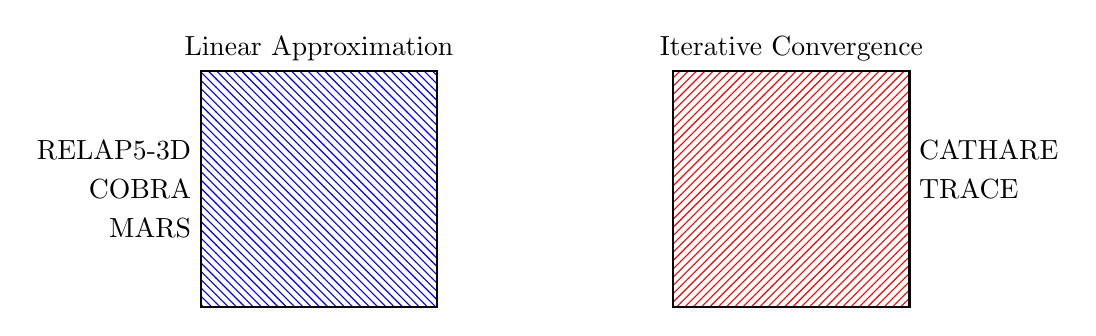
\begin{tikzpicture}
\draw[pattern=north west lines, pattern color=blue] [thick] (-3,0) rectangle (0,3);
\draw (-1.5,3) node[anchor=south] {Linear Approximation};
\draw (-3,2) node[anchor=east] {RELAP5-3D};
\draw (-3,1.5) node[anchor=east] {COBRA};
\draw (-3,1) node[anchor=east] {MARS};
\draw[pattern=north east lines, pattern color=red] [thick] (3,0) rectangle (6,3);
\draw (4.5,3) node[anchor=south] {Iterative Convergence};
\draw (6,2) node[anchor=west] {CATHARE};
\draw (6,1.5) node[anchor=west] {TRACE};
\end{tikzpicture}
}
\end{figure}

\end{frame}
%------------------------------------------------
%------------------------------------------------
\subsection[Research Objectives]{Research Objectives}
%---------
%---------
\begin{frame}
\frametitle{Research Objectives}

\begin{figure}[t]
\centering
\resizebox{!}{0.7\textheight}{
\tikzsetnextfilename{images/my_diagram_eps}
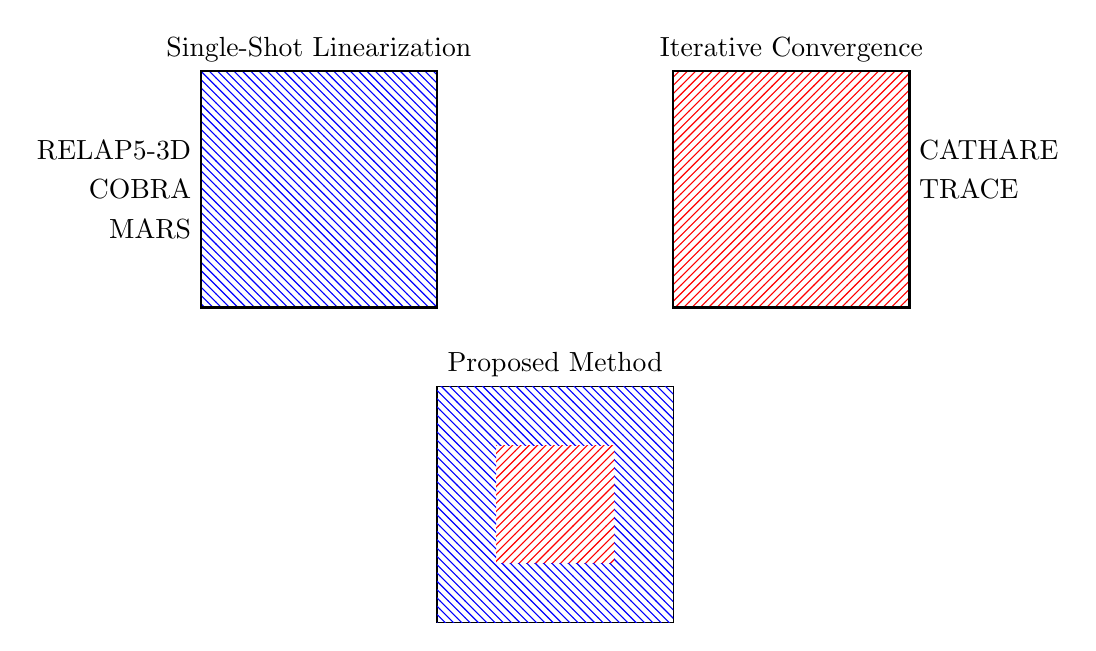
\begin{tikzpicture}
\draw[pattern=north west lines, pattern color=blue] [thick] (-3,0) rectangle (0,3);
\draw (-1.5,3) node[anchor=south] {Single-Shot Linearization};
\draw (-3,2) node[anchor=east] {RELAP5-3D};
\draw (-3,1.5) node[anchor=east] {COBRA};
\draw (-3,1) node[anchor=east] {MARS};
\draw[pattern=north east lines, pattern color=red] [thick] (3,0) rectangle (6,3);
\draw (4.5,3) node[anchor=south] {Iterative Convergence};
\draw (6,2) node[anchor=west] {CATHARE};
\draw (6,1.5) node[anchor=west] {TRACE};
\draw (0,-4) rectangle +(3,3);
\path[pattern=north west lines, pattern color=blue] (0,-4) rectangle +(0.75,3);
\path[pattern=north west lines, pattern color=blue] (2.25,-4) rectangle +(0.75,3);
\path[pattern=north west lines, pattern color=blue] (0.75,-1.75) rectangle +(1.5,0.75);
\path[pattern=north east lines, pattern color=red] (0.75,-3.25) rectangle +(1.5,1.5);
\path[pattern=north west lines, pattern color=blue] (0.75,-4) rectangle +(1.5,0.75);
\draw (1.5,-1) node[anchor=south] {Proposed Method};
\end{tikzpicture}
}
\end{figure}

\end{frame}
%------------------------------------------------------------------------------
%------------------------------------------------------------------------------
\section[Nonlinear]{Nonlinear Solver}
%------------------------------------------------
%------------------------------------------------
\subsection[Nonlinear Algorithm]{Nonlinear Algorithm}
%---------
%---------
\begin{frame}
\frametitle{Nonlinear Solver: Momentum Flow Paths, $\vec{F}^{k}_{p}$}
\begin{equation*}
\frac{\partial\, \vec{F}^{k}_{p}}{\partial \dot{m}^{n+1}_{l}} \delta \dot{m}_{l}^{k} + \frac{\partial\, \vec{F}^{k}_{p}}{\partial \dot{m}^{n+1}_{g}} \delta \dot{m}_{g}^{k} + \frac{\partial\, \vec{F}^{k}_{p}}{\partial \dot{m}^{n+1}_{e}} \delta \dot{m}_{e}^{k} + \sum_{i\, \in \, N_{c}} \frac{\partial\, \vec{F}^{k}_{p}}{\partial P_{i}} \delta P_{i}^{k} = - \vec{F}^{k}_{p}
\end{equation*}

\begin{equation*}
\vec{J}^{k}_{p} \delta \momVec{}^{k}  = - \vec{F}^{k}_{p} - \sum_{i\, \in \, N_{c}} \frac{\partial\, \vec{F}^{k}_{p}}{\partial P_{i}} \delta P_{i}^{k}
\end{equation*}

\begin{equation*}
\delta \momVec{}^{k} = - \left[\vec{J}_{p}^{k}\right]^{-1} \left[\vec{F}^{k}_{p} \right] - \sum_{i \, \in \, N_{c} } \left[\vec{J}^{k}_{p}\right]^{-1} \left[\frac{\partial \vec{F}^{k}_{p}}{\partial P_{i}}\right] \delta P^{k}_{i}
\end{equation*}

\begin{equation*}
\delta \momVec{}^{k} = \delta \momVec{}^{*} + \sum_{i \, \in \, N_{c} } \frac{\partial \momVec{}^{k}}{\partial P_{i}} \delta P^{k}_{i}
\end{equation*}

\end{frame}
%---------
%---------
\begin{frame}[shrink=25]
\frametitle{Nonlinear Solver: Continuity Volumes, $\vec{F}^{k}_{c}$}

\begin{IEEEeqnarray*}{lcr}
\frac{\partial \vec{F}^{k}_{c}}{\partial (\alpha_{g} P_{n} )} \delta (\alpha_{g} P_{n})^{k} + \frac{\partial \vec{F}^{k}_{c}}{\partial \alpha_{g}} \delta \alpha^{k}_{g} + \frac{\partial \vec{F}^{k}_{c}}{\partial (\alpha_{g} h_{v} )} \delta (\alpha_{g} h_{v})^{k} +
\frac{\partial \vec{F}^{k}_{c}}{\partial ((1 - \alpha_{g}) h_{l} )} \delta ((1 - \alpha_{g}) h_{l})^{k} & & \nonumber \\
 + \frac{\partial \vec{F}^{k}_{c}}{\partial \alpha_{e}} \delta \alpha_{e}^{k} + \frac{\partial \vec{F}^{k}_{c}}{\partial P } \delta P^{k} + \sum_{i \, \in \, N_{f} } \frac{\partial \vec{F}^{k}_{c}}{\partial \momVec{}_{i} } \delta \momVec{}_{i}^{k}  = - \vec{F}^{k}_{c} & & \nonumber
\end{IEEEeqnarray*}

\begin{equation*}
\frac{\partial \vec{F}_{c}^{k}}{\partial \momVec{}_{i}} = \vec{\Xi}^{k}_{i} = \dt{} \begin{bmatrix}
 0 & \frac{\don{\alpha^{n}_{g} \rho^{n}_{n}}^{n+1,k}_{d}}{\ave{\alpha_{g} \rho_{g}}^{n}_{a}} & 0 \\
\frac{\don{\alpha^{n}_{l}\rho^{n}_{l}}^{n+1,k}_{d}}{\ave{\alpha_{l} \rho_{l}}^{n}_{a}} & 0 & 0 \\
0 & \frac{\don{\alpha^{n}_{g} \rho^{n}_{g} h^{n}_{g}}^{n+1,k}_{d}}{\ave{\alpha_{g} \rho_{g}}^{n}_{a}} & 0 \\
\frac{\don{\alpha^{n}_{l}\rho^{n}_{l} h^{n}_{l}}^{n+1,k}_{d}}{\ave{\alpha_{l} \rho_{l}}^{n}_{a}} & 0 & \frac{\don{\alpha^{n}_{e} \rho^{n}_{l} h^{n}_{l}}^{n+1, k}_{d}}{\ave{\alpha_{e} \rho_{l}}^{n}_{a}} \\
0 & 0 & \frac{ \don{\alpha^{n}_{e} \rho^{n}_{l}}^{n+1, k}_{d}}{ \ave{\alpha_{e} \rho_{l}}^{n}_{a}} \\
0 & \frac{ \don{\alpha^{n}_{g} \rho^{n}_{v}}^{n+1, k}_{d}}{ \ave{\alpha_{g} \rho_{g}}^{n}_{a}} & 0
\end{bmatrix}_{i}
\end{equation*}


\end{frame}
%---------
%---------
\begin{frame}[shrink=25]
\frametitle{Nonlinear Solver: Collapse Equations}

\begin{IEEEeqnarray}{rcl}
\frac{\partial \vec{F}^{k}_{c}}{\partial (\alpha_{g} P_{n} )} \delta (\alpha_{g} P_{n})^{k} + \frac{\partial \vec{F}^{k}_{c}}{\partial \alpha_{g}} \delta \alpha^{k}_{g} + \frac{\partial \vec{F}^{k}_{c}}{\partial (\alpha_{g} h_{v} )} \delta (\alpha_{g} h_{v})^{k} + \frac{\partial \vec{F}^{k}_{c}}{\partial ((1 - \alpha_{g}) h_{l} )} \delta ((1 - \alpha_{g}) h_{l})^{k} & + & \nonumber \\
\frac{\partial \vec{F}^{k}_{c}}{\partial \alpha_{e}} \delta \alpha_{e}^{k} + \frac{\partial \vec{F}^{k}_{c}}{\partial P } \delta P^{k} + \sum_{i\, \in \, N_{f} } \vec{\Xi}^{k}_{i}\left( \delta \momVec{}_{i}^{*} + \frac{\partial \momVec{}_{i}^{k}}{\partial P_{s(i)}} \delta P_{s(i)}^{k} + \frac{\partial \momVec{}_{i}^{k}}{\partial P_{o(i)}} \delta P_{o(i)}^{k} \right) = \vec{F}^{k}_{c} & &\nonumber
\end{IEEEeqnarray}

\begin{IEEEeqnarray}{rcl}
\frac{\partial \vec{F}^{k}_{c}}{\partial (\alpha_{g} P_{n} )} \delta (\alpha_{g} P_{n})^{k} + \frac{\partial \vec{F}^{k}_{c}}{\partial \alpha_{g}} \delta \alpha^{k}_{g} + \frac{\partial \vec{F}^{k}_{c}}{\partial (\alpha_{g} h_{v} )} \delta (\alpha_{g} h_{v})^{k} + \frac{\partial \vec{F}^{k}_{c}}{\partial ((1 - \alpha_{g}) h_{l} )} \delta ((1 - \alpha_{g}) h_{l})^{k} & + & \nonumber \\
\frac{\partial \vec{F}^{k}_{c}}{\partial \alpha_{e}} \delta \alpha_{e}^{k} + \left( \frac{\partial \vec{F}^{k}_{c}}{\partial P } + \sum_{i\,\in \, N_{f} } \vec{\Xi}^{k}_{i}\frac{\partial \momVec{}^{k}_{i}}{\partial P_{s(i)}}\right) \delta P^{k} + \sum_{i \, \in \, N_{f} } \vec{\Xi}^{k}_{i} \frac{\partial \momVec{}_{i}^{k}}{\partial P_{o(i)}} \delta P_{o(i)}^{k} & = & \nonumber \\
- \vec{F}^{k}_{c} - \sum_{i \, \in \, N_{f} } \vec{\Xi}^{k}_{i} \delta \momVec{}_{i}^{*} \nonumber & &
\end{IEEEeqnarray}

\end{frame}
%---------
%---------
\begin{frame}[shrink=25]
\frametitle{Nonlinear Solver: Assemble, Solve and Update}

\begin{columns}
\column{0.75\textwidth}
\begin{IEEEeqnarray}{rcl}
\left[ \vec{J}^{k}_{c} \vert \vec{K}^{k}_{c} \right] \delta \vec{C}_{c}^{k} & = &  \vec{r}^{k}_{c} \nonumber \\
\left[ \vec{U}^{k}_{c} \vert \left[\vec{L}^{k}_{c}\right]^{-1}\vec{K}^{k}_{c} \right] \delta \vec{C}^{k}_{c} & = & \left[\vec{L}^{k}_{c}\right]^{-1}\vec{r}^{k}_{c} \nonumber
\end{IEEEeqnarray}

Each continuity volume contributes its conservation of vapor mass equation to a global matrix that solves for the pressure updates of each continuity volume.

\begin{equation*}
\vec{A}^{k}\delta \vec{P}^{k} = \vec{res}^{k}
\end{equation*}

After the pressure update is obtained, each continuity volume and momentum flow path is traversed to calculate their respective updates.

\column{0.25\textwidth}

\begin{equation*}
\delta \vec{C}_{c} \equiv 
\begin{bmatrix}
\delta ( \alpha_{g} P_{n} ) \\
\delta \alpha_{g} \\
\delta ( \alpha_{g} h_v ) \\
\delta ( (1 - \alpha_{g} ) h_l ) \\
\delta \alpha_{e} \\
\delta P \\ 
\delta P_{o(1)} \\
\vdots \\
\delta P_{o(N_{f})}
\end{bmatrix}
\end{equation*}

\end{columns}

\end{frame}
%---------
%---------
\begin{frame}[shrink=1]
\frametitle{Nonlinear Solver: Convergence Determination}

The determination of nonlinear convergence is based upon three conditions.

\begin{IEEEeqnarray}{rclcrcl}
\frac{||\tilde{\vec{F}}^{k+1}||_{2}}{\sqrt{N_{u}}} \, & \leq & \, \ftol{} & \quad & \tilde{\vec{F}}^{k} &=& \left[\vec{S}^{k}\right]^{-1}\vec{F}^{k}\nonumber \\
\frac{||\delta \tilde{\vec{x}}^{k}||_{2}}{\sqrt{N_{u}}}  \, & \leq & \, \dtol{} & \quad & \delta \tilde{\vec{x}}^{k} &=& \frac{\delta \vec{x}^{k}}{\vec{x}^{n+1, k}} = \frac{ \vec{x}^{n+1, k+1} - \vec{x}^{n+1, k}}{\vec{x}^{n+1,k}} \nonumber \\
k \, & > & \, \kmax & \quad & & &\nonumber 
\end{IEEEeqnarray}

The nonlinear convergence parameters for this work, unless otherwise stated, are \kmax{} = 35, $F_{\text{tol}}$ = \expneg{1.0}{6}, $\delta_{\text{tol}}$ = \expneg{1.0}{8}.

\end{frame}
%------------------------------------------------
%------------------------------------------------
\subsection[Operator-Based Scaling]{Operator-Based Scaling}
%---------
%---------
\begin{frame}
\frametitle{Operator-Based Scaling: Intent}

Scaled residual:
\begin{equation*}
\tilde{\vec{F}}^{k} = \left[\vec{S}^{k}\right]^{-1}\vec{F}^{k}\end{equation*}

\begin{itemize}
\item{$\left( S_{i}^{-1} F_{i} \right)^{k} \approx 1$ when $\vec{x}^{k}$ is a "poor" solution.}
\item{$(S_{i}^{-1} F_i)^{k} \approx 0$ when $\vec{x}^{k}$ is a "good" solution.}
\item{$\left( S_{i}^{-1} F_{i} \right)^{k} \rightarrow 0$ when phase $i$ disappears.}
\item{$0 \leq \abs{ \left( S_{i}^{-1} F_{i} \right)^{k} } \leq 1 $ for all values of $\vec{x}^{k}_i$.}
\end{itemize}

At low volume fractions:
\begin{equation*}
S_{\phi} = \max[1.0, \left(C_{1}\frac{\alpha_{\phi,\text{min}}}{\alpha_{\phi}}\right)^{C_{2}} ] S_{\phi}
\end{equation*}

\end{frame}
%---------
%---------
\begin{frame}
\frametitle{Operator-Based Scaling: Balance Equations}


\end{frame}
%---------
%---------
\begin{frame}[shrink=5]
\frametitle{Operator-Based Scaling: Examples}

\begin{IEEEeqnarray}{rcl}
S^{k}_{m,l} & = & V_c \abs{\left(\alpha_l \rho_l \right)^{n+1,k} - \left(\alpha_l \rho_l \right)^{n}} + \dt{} \sum_{i\,\in\,N_{f}}\abs{\don{\alpha^n_l \rho^n_l}^{n+1,k}_{d} u^{n+1,k}_l  A_{m}}_{i} \nonumber \\
&+& \abs{(1-\eta)\Gamma}^{n+1,k} + \abs{\Upsilon}^{n+1,k} \nonumber \\
S^{k}_{p, l} & = & \frac{\dt{}}{\dx{}} \left[\abs{\frac{\dx{} \left[\dot{m}_{l}^{n+1, k} - \dot{m}_{l}^{n}\right]}{\dt{}}} + \abs{\sum_{i\, \in \, N_{c} } \left( \don{\alpha_l \rho_l u_l}_{\text{d}} \ave{u}_{\text{a},l} \tilde{A}\right)^{n}_{i}} \right. \nonumber \\ 
& + & \abs{\ave{\alpha_l}^{n}_{\text{a}} \nabla P^{\,n+1, k}} + \abs{g \ave{\alpha_l \rho_l}_{\text{a}}^{n}} + \abs{K^{n}_{wl}(\dot{m}_l^{n+1, k})^2} \nonumber \\
& + & \abs{K^{n}_{i,gl}(u^{n+1, k}_{l} - u^{n+1,k}_{g})^2} + \abs{(1 - \eta)\dot{\Gamma} u^{'}}^{n} + \abs{\dot{\Upsilon} u^{'}}^{n} \left. \vphantom{\abs{\frac{\dx{} \left[\dot{m}_{l}^{n+1, k} - \dot{m}_{l}^{n}\right]}{\dt{}}}}  \right] \nonumber
\end{IEEEeqnarray}

\end{frame}
%------------------------------------------------
%------------------------------------------------
\subsection[Implementation \& Efficacy]{Implementation and Efficacy}
%---------
%---------
\begin{frame}
\frametitle{Timestep Sensitivity}

Timestep size sensitivity studies with the set of \dtmax{} given by
\begin{equation*}
\dtmax{} \in \bigcup^{n_{t}-1}_{i\, = 0} \frac{\dt{}_{0}}{r^{i}_{f}}
\end{equation*}

For the following two problems, $n_{t}$ = 6, $r_{f}$ = 10, and $\dtmax{}_{o}$ = 1.0 [s]. 

\end{frame}
%---------
%---------
\begin{frame}
\frametitle{Single-Phase and Flashing Problems}
\begin{columns}
\column{0.78\textwidth}

\textbf{Purpose:} to test the implementation of the nonlinear solver and to determine its efficacy.

\begin{itemize}
\item{Cross-sectional area: 4 [in$^2$]}
\item{\dx{} is constant: 4 [in]}
\item{IC: Single-Phase: $\alpha_{l} = 1$, @ 200 [psia].}
\item{IC: Flashing: $\alpha_{g}=1$, @ 200 [psia].}
\item{Outlet Conditions $\longleftrightarrow$ Initial Conditions.}
\item{Inlet Conditions: $\alpha_{l}=1$, @ 200 \& 1000 [psia].}
\end{itemize}
\begin{equation*}
\dot{m}(t) = \left\{
\begin{array}{cclrcll}
 0.0           & [\frac{ \lbm{} }{\text{s}}] & , &                & t & \leq 1 & [\text{s}] \\
 0.5 ( t - 1)  & [\frac{ \lbm{} }{\text{s}}] & , & 1\; [\text{s}] < & t & \leq 2 & [\text{s}] \\
 0.5           & [\frac{ \lbm{} }{\text{s}}] & , &                & t & > 2    & [\text{s}]
\end{array}\right.
\end{equation*}

\column{0.22\textwidth}
\begin{figure}[h!t]
\centering
\resizebox{\textwidth}{0.6\textheight}{
\tikzsetnextfilename{images/dualModel_pdf}
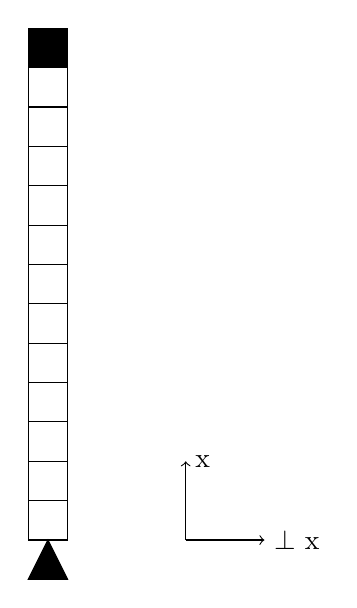
\begin{tikzpicture}
\foreach \x in {1,..., 12} \draw(0, 0.5*\x-0.5) rectangle +(.5,.5);
\filldraw[fill=black] (0, 6) rectangle +(.5,.5); 
\filldraw[fill=black] (0, -0.5) -- (0.25, 0) -- (0.5, -0.5) -- cycle;
\draw[->] (2,0) -- (2, 1) node[anchor=west] {x};
\draw[->] (2,0) -- (3, 0) node[anchor=west] {$\perp$ x};
\end{tikzpicture}
}

\end{figure}
\end{columns}
\end{frame}
%---------
%---------
\begin{frame}
\frametitle{Single-Phase Solution with $\dtmax{} = \expneg{1.0}{0}$ [s]}

\begin{figure}[h!t]
\centering
\includegraphics[width=0.94\textwidth]{../plots/single1pt000em0_pdf}
\end{figure}

\end{frame}
%---------
%---------
\begin{frame}
\frametitle{Single-Phase Solution with $\dtmax{} = \expneg{1.0}{5}$ [s]}

\begin{figure}[h!t]
\centering
\includegraphics[width=0.94\textwidth]{../plots/single1pt000em5_pdf}
\end{figure}

\end{frame}
%---------
%---------
\begin{frame}
\frametitle{Flashing Solution at $\dtmax{} = \expneg{1.0}{0}$ [s]}

\begin{figure}[h!t]
\centering
\includegraphics[width=0.94\textwidth]{../plots/flashing1pt0000em0_pdf}
\end{figure}

\end{frame}
%---------
%---------
\begin{frame}
\frametitle{Flashing Solution at $\dtmax{} = \expneg{1.0}{5}$ [s]}

\begin{figure}[h!t]
\centering
\includegraphics[width=0.94\textwidth]{../plots/flashing1pt0000em5_pdf}
\end{figure}

\end{frame}
%---------
%---------
\begin{frame}
\frametitle{Linear Solver's Timestep Size Insensitive Solution}

\begin{figure}[h!t]
\centering
\includegraphics[width=.94\textwidth]{../plots/flashingDtInsensitiveLin_pdf}
\end{figure}

\end{frame}
%---------
%---------
\begin{frame}
\frametitle{Nonlinear Solver's Timestep Size Insensitive Solution}

\begin{figure}[h!t]
\centering
\includegraphics[width=.94\textwidth]{../plots/flashingDtInsensitiveNln_pdf}
\end{figure}

\end{frame}
%---------
%---------
\begin{frame}
\frametitle{Flashing Residual from Linear Solver}

\begin{figure}[h!t]
\centering
\includegraphics[width=0.94\textwidth]{../plots/flashingResidualLin_pdf}
\end{figure}

\end{frame}
%---------
%---------
\begin{frame}
\frametitle{Flashing Residual from Nonlinear Solver}

\begin{figure}[h!t]
\centering
\includegraphics[width=0.94\textwidth]{../plots/flashingResidualNln_pdf}
\end{figure}

\end{frame}
%------------------------------------------------------------------------------
%------------------------------------------------------------------------------
\section[SNR]{Selective Nonlinear Refinement}
%------------------------------------------------
%------------------------------------------------
\subsection[Domain Decomposition Algorithm]{Domain Decomposition Algorithm}
%---------
%---------
\begin{frame}[shrink=25]
\frametitle{Domain Decomposition: The Boundaries}
On the linear side of the linear-nonlinear domain boundary, the flow rates connecting the two domains are kept as unknowns.

\begin{IEEEeqnarray}{rcl}
\frac{\partial \vec{F}^{k}_{c}}{\partial (\alpha_{g} P_{n} )} \delta (\alpha_{g} P_{n})^{k} + \frac{\partial \vec{F}^{k}_{c}}{\partial \alpha_{g}} \delta \alpha^{k}_{g} + \frac{\partial \vec{F}^{k}_{c}}{\partial (\alpha_{g} h_{v} )} \delta (\alpha_{g} h_{v})^{k} + \frac{\partial \vec{F}^{k}_{c}}{\partial ((1 - \alpha_{g}) h_{l} )} \delta ((1 - \alpha_{g}) h_{l})^{k} & + &  \nonumber \\
\frac{\partial \vec{F}^{k}_{c}}{\partial \alpha_{e}} \delta \alpha_{e}^{k} + \frac{\partial \vec{F}^{k}_{c}}{\partial P } \delta P^{k} + \sum_{i \, \in \, N_{f} } \frac{\partial \vec{F}^{k}_{c}}{\partial \momVec{}_{i} } \delta \momVec{}_{i}^{k} + \sum_{i\,\in \, N_{\text{NBC}}} \frac{\partial \vec{F}^{k}_{c}}{\partial \vec{\Psi}_{i} } \delta \vec{\Psi}_{i}^{k}  = - \vec{F}^{k}_{c} & &\nonumber 
\end{IEEEeqnarray}

\begin{IEEEeqnarray}{rcl}
\frac{\partial \vec{F}^{k}_{c}}{\partial (\alpha_{g} P_{n} )} \delta (\alpha_{g} P_{n})^{k} + \frac{\partial \vec{F}^{k}_{c}}{\partial \alpha_{g}} \delta \alpha^{k}_{g} + \frac{\partial \vec{F}^{k}_{c}}{\partial (\alpha_{g} h_{v} )} \delta (\alpha_{g} h_{v})^{k} + \frac{\partial \vec{F}^{k}_{c}}{\partial ((1 - \alpha_{g}) h_{l} )} \delta ((1 - \alpha_{g}) h_{l})^{k} & + & \nonumber \\
\frac{\partial \vec{F}^{k}_{c}}{\partial \alpha_{e}} \delta \alpha_{e}^{k} + \left( \frac{\partial \vec{F}^{k}_{c}}{\partial P } + \sum_{i \, \in \, N_{f} } \vec{\Xi}^{k}_{i}\frac{\partial \momVec{}^{k}_{i}}{\partial P}\right) \delta P^{k} + \sum_{i \, \in \, N_{f} } \vec{\Xi}^{k}_{i} \frac{\partial \momVec{}_{i}^{k}}{\partial P_{o(i)}} \delta P_{o(i)}^{k} + \dt{} \sum_{i \, \in \, N_{\text{NBC}}} \delta \vec{\Psi}^{k}_{i} & = &\nonumber \\
- \left( \vec{F}^{k}_{c} + \sum_{i \, \in \, N_{f} } \vec{\Xi}^{k}_{i} \delta \momVec{}_{i}^{*} - \dt{} \sum_{i \, \in \, N_{\text{NBC}}} \vec{\Psi}^{k}_{i} \right) - \dt{} \sum_{i \, \in \, N_{\text{NBC}}} \vec{\Psi}^{k}_{i} & & \nonumber
\end{IEEEeqnarray}

%\begin{equation*}
%\left[ \vec{J}_{n} \vert \vec{K}_{n} \vert \vec{Q}_{n} \right] \delta \vec{C}_{n} = \vec{r}_{n} - \vec{Q}_{n} \vec{\Psi}_{n}
%\end{equation*}

\end{frame}
%---------
%---------
\begin{frame}[shrink=25]
\frametitle{Linear Pressure Matrix}

\begin{columns}
\column{0.75\textwidth}

\begin{IEEEeqnarray}{rcl}
\left[ \vec{J}_{n} \vert \vec{K}_{n} \vert \vec{Q}_{n} \right] \delta \vec{C}_{n} &=& \vec{r}_{n} - \vec{Q}_{n} \vec{\Psi}_{n} \nonumber \\
\left[ \vec{U}_{n} \vert \vec{L}^{-1}_{n}\vec{K}_{n} \vert \vec{L}^{-1}_{n}\vec{Q}_{n} \right] \delta \vec{C}_{j} & = & \vec{L}^{-1}_{n}\vec{r}_{n}  -\vec{L}^{-1}_{n}\vec{Q}_{n}\vec{\Psi}_{n} \nonumber 
\end{IEEEeqnarray}

Linear domain's pressure matrix is now:

\begin{IEEEeqnarray}{rcl}
\vec{A}_{\text{lin}} \delta \vec{P}_{\text{lin}} + \vec{B}_{\text{lin}} \delta \vec{\Psi}_{\text{lin}} & = & \vec{res}_{\text{lin}} - \vec{B}_{\text{lin}} \vec{\Psi}_{\text{lin}} \nonumber \\
\delta \vec{P}_{\text{lin}} + \vec{A}^{-1}_{\text{lin}}\vec{B}_{\text{lin}} \delta \vec{\Psi}_{\text{lin}} & = & \vec{A}^{-1}_{\text{lin}}\vec{res}_{\text{lin}} - \vec{A}^{-1}_{\text{lin}}\vec{B}_{\text{lin}} \vec{\Psi}_{\text{lin}} \nonumber \\
\delta \vec{P}_{\text{lin}} + \vec{W}_{\text{lin}} \delta \vec{\Psi}_{\text{lin}} & = & \delta \vec{P}^{*}_{\text{lin}} - \vec{W}_{\text{lin}} \vec{\Psi}_{\text{lin}} \nonumber
\end{IEEEeqnarray}

The row's from the linear pressure matrix that correspond to the nonlinear boundary continuity volumes are:

\begin{equation*}
\delta P_{j} + \sum_{i\, \in \, N_{n}} \vec{w}^{T}_{j, i} \cdot \delta \vec{\Psi}_{i} = \delta P_{j}^{*} - \sum_{i\, \in \, N_{n}} \vec{w}^{T}_{j, i} \cdot{} \vec{\Psi}^{k}_{i}
\end{equation*}

\column{0.25\textwidth}

\begin{equation*}
\delta \vec{C}_{n} =
\begin{bmatrix}
\delta ( \alpha_{g} P_{n} ) \\
\delta \alpha_{g} \\
\delta ( \alpha_{g} h_v ) \\
\delta ( (1 - \alpha_{g} ) h_l ) \\
\delta \alpha_{e} \\
\delta P \\ 
\delta P_{o(1)} \\
\vdots \\
\delta P_{o(N_{f})} \\
\delta \vec{\Psi}_{1} \\
\vdots \\
\delta \vec{\Psi}_{N_{\text{NBC}}}
\end{bmatrix}
\end{equation*}

\end{columns}

\end{frame}
%---------
%---------
\begin{frame}[shrink=25]
\frametitle{Nonlinear Pressure Matrix}

The flow rates is these equations are expressed in terms of the momenta. 

\begin{equation*}
\vec{\Psi}^{n+1, k}_{i} = \vec{\Xi}^{n+1, k}_{i} \cdot \vec{\dot{m}}^{n+1, k}_{i}
\end{equation*}

The pressure equations for the NBC volumes are then added to the nonlinear domain's pressure matrix.

\begin{IEEEeqnarray}{rcl}
\delta P_{j} + \sum_{i\,\in \, N_{n}} \vec{w}^{T}_{j,i} \vec{\Xi}^{k}_{i} \delta \vec{m}^{k}_{i} & = & \delta P^{*}_{j} - \sum_{i\,\in \, N_{n}} \vec{w}^{T}_{j,i} \vec{\Xi}_{i}^{k} \momVec{}^{k}_{i}  \nonumber \\
\delta P_{j} + \sum_{i\,\in \, N_{n}} \vec{w}^{T}_{j,i} \left[\vec{\Xi}_{i}^{k} \frac{\partial \momVec{}_{i}^{k}}{\partial P_{s(i)}} \delta P_{s(i)} + \vec{\Xi}_{i}^{k} \frac{\partial \momVec{}_{i}^{k}}{\partial P_{o(i)}} \delta P_{o(i)}\right] & = & \delta P^{*}_{j} - \sum_{i\,\in \, N_{n}} \vec{w}^{T}_{j,i} \left[ \vec{\Xi}_{i}^{k} \momVec{}^{k}_{i} + \vec{\Xi}_{i}^{k}\delta \momVec{}^{*}_{i} \right] \nonumber
\end{IEEEeqnarray}

The nonlinear pressure matrix is inverted to obtain updates to the nonlinear domain's pressures.

\begin{equation*}
\vec{A}^{k}_{\text{nln}} \delta \vec{P}^{k}_{\text{nln}} = \vec{res}^{k}_{\text{nln}}
\end{equation*}

Once the nonlinear domain is converged, the linear domain's pressure updates are obtained.

\begin{equation*}
\delta P_{j} = \delta P^{*}_{j} - \sum_{i\,\in \, N_{n}} \vec{w}_{j,i}^{T} \vec{\Xi}^{k}_{i} \left[ \momVec{}^{k}_{i} + \delta \momVec{}_{i}\right]
\end{equation*}


\end{frame}
%------------------------------------------------
%------------------------------------------------
\subsection[Implementation \& Efficacy]{Implementation and Efficacy}
%---------
%---------
\begin{frame}
\frametitle{Complex Geometry}

\textbf{Purpose:} to test the implementation of the domain decomposition algorithm.

\begin{columns}
\column{0.7\textwidth}

\begin{itemize}
\item{Model of GE experimental facility.}
\item{3 x 3 rod bundle.}
\item{3 sections.}
\item{18 subchannels.}
\item{56 inter-subchannel flow paths.}
\item{256 different simulations.}
\item{Error = $\displaystyle \sum_{i\,=\,1}^{N_{t}} \abs{P_{\text{lin}}(t^{i}) -P_{k}(t^{i})}$.}
\end{itemize}

\column{0.4\textwidth}

\begin{figure}[h!t]
\centering
\resizebox{\textwidth}{!}{
\begin{center}
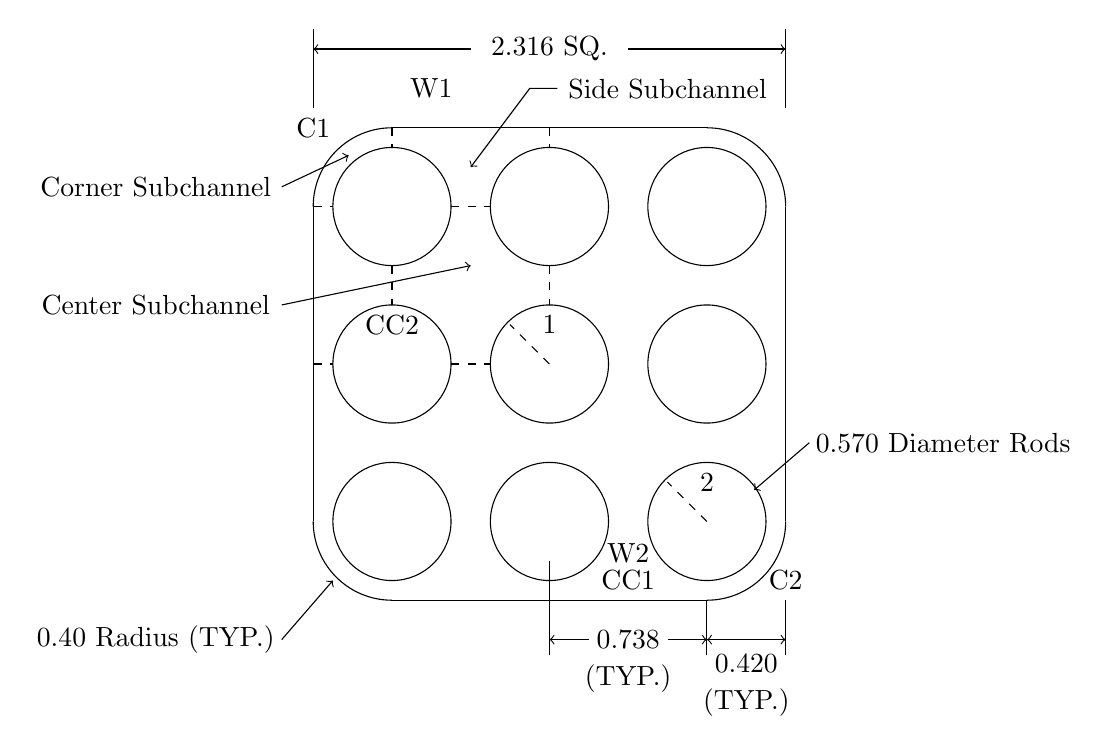
\begin{tikzpicture}

%Rounded corners
\draw (3,2) arc (0:90:1);
\draw (-2,3) arc (90:180:1);
\draw (-3,-2) arc (180:270:1);
\draw (2,-3) arc (270:360:1);

%Grid of circles
\draw (0,0) circle (0.75);
\draw (0,2) circle (0.75);
\draw (0,-2) circle (0.75);
\draw (2,0) circle (0.75);
\draw (2,2) circle (0.75);
\draw (2,-2) circle (0.75);
\draw (-2,0) circle (0.75);
\draw (-2,2) circle (0.75);
\draw (-2,-2) circle (0.75);

%Box
\draw (-3,-2) -- (-3,2);
\draw (3,-2) -- (3,2);
\draw (2,-3) -- (-2,-3);
\draw (-2,3) -- (2,3);

%Misc lines
\draw [dashed] (-2,3) -- (-2,2.75);
\draw [dashed] (0,3) -- (0,2.75);
\draw [dashed] (-2,1.25) -- (-2,0.75);
\draw [dashed] (0,1.25) -- (0,0.75);
\draw [dashed] (-3,2) -- (-2.75,2);
\draw [dashed] (-3,0) -- (-2.75,0);
\draw [dashed] (-1.25,2) -- (-0.75,2);
\draw [dashed] (-1.25,0) -- (-0.75,0);

\draw [dashed] (0,0) -- (-0.5,0.5);
\draw [dashed] (2,-2) -- (1.5,-1.5);

%Misc arrows and labels
\draw [<-] (-3,4) -- (-1,4);
\draw [->] (1,4) -- (3,4);
\draw (-3,4.25) -- (-3,3.25);
\draw (3,4.25) -- (3,3.25);
\draw (0,4) node {2.316 SQ.};

\draw [<-] (0,-3.5) -- (0.5,-3.5);
\draw [->] (1.5,-3.5) -- (2,-3.5);
\draw (2,-3.7) -- (2,-3);
\draw (0,-3.7) -- (0,-2.5);
\draw (1,-3.5) node {0.738};
\draw (1,-4) node {(TYP.)};

\draw [<->] (2,-3.5) -- (3,-3.5);
\draw (3,-3.7) -- (3,-3);
\draw (2.5,-3.8) node {0.420};
\draw (2.5,-4.3) node {(TYP.)};

\draw [->] (-3.4,2.25) -- (-2.55,2.65);
\draw (-5,2.25) node {Corner Subchannel};

\draw [->] (-3.4,0.75) -- (-1,1.25);
\draw (-5,0.75) node {Center Subchannel};

\draw [->] (0.1,3.5) -- (-0.25,3.5) -- (-1,2.5);
\draw (1.5,3.5) node {Side Subchannel};

\draw [->] (-3.4,-3.5) -- (-2.75,-2.75);
\draw (-5,-3.5) node {0.40 Radius (TYP.)};

\draw [->] (3.3,-1) -- (2.6,-1.6);
\draw (5,-1) node {0.570 Diameter Rods};

\draw (-3,3) node {C1};
\draw (-1.5,3.5) node {W1};
\draw (1,-2.75) node {CC1};

\draw (3,-2.75) node {C2};
\draw (1,-2.4) node {W2};
\draw (-2,0.5) node {CC2};

\draw (0,0.5) node {1};
\draw (2,-1.5) node {2};

\end{tikzpicture}
\end{center}
\caption{Position of pressure taps for setting isokinetic conditions. Note splitter positions for the various subchannels.}
\label{fig:position_of_pressure taps}
}
\end{figure}

\end{columns}
\end{frame}
%---------
%---------
\begin{frame}
\frametitle{Error in Complex Geometry Problem}

\begin{figure}[h!t]
\centering
\includegraphics[width=0.94\textwidth]{../plots/complexBar_pdf}
\end{figure}

\end{frame}
%---------
%---------
\begin{frame}
\frametitle{Valve Problem}

\textbf{Purpose:} to determine efficacy of the selective nonlinear refinement algorithm.

\begin{itemize}
\item{Four 40 [in] subchannels: $A_{c} = 16$ [in$^{2}$], \dx{} = 5 [in].}
\item{Conditions:
	\begin{itemize}
	\item{Initial $\rightarrow$ $\alpha_{l} = 1$ @ 800 [psia].}
	\item{Inlet $\rightarrow$ $\alpha_{l} = 1$ @ 818 [psia].}
	\item{Outlet $\rightarrow$ $\alpha_{l} = 1$ @ 800 [psia].}
	\end{itemize}
}
\item{Obstructions @ 15 [in]:
\begin{itemize}
	\item{Subchannel 1 $\rightarrow$ K = $\infty$ [-].}
	\item{Subchannel 2 $\rightarrow$ K = 40 [-].}
	\item{Subchannel 3 $\rightarrow$ K = 160 [-].}
	\item{Subchannel 4 $\rightarrow$ K(t) $\rightarrow K(t) = \frac{K_{o}}{{A(t)_r}^2}$, $K_{o} = 10$ [-].}
\end{itemize}
}
\item{No connections between channels.}
\end{itemize}

\end{frame}
%---------
%---------
\begin{frame}
\frametitle{Valve Problem Model}

\begin{center}
\resizebox{0.75\textwidth}{0.75\textheight}{
\tikzsetnextfilename{images/valveModel_pdf}
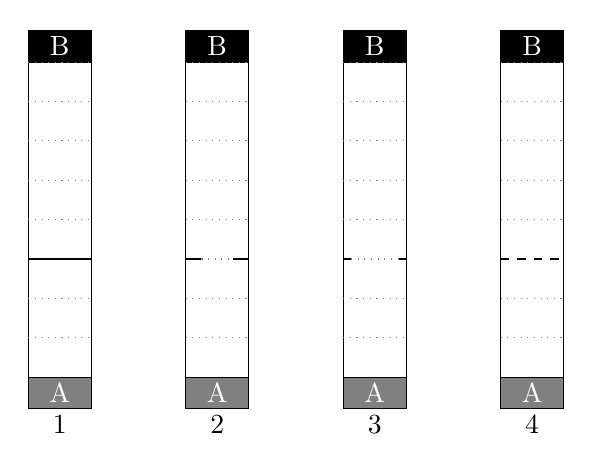
\begin{tikzpicture}
\foreach \x in {-3,-1,1,3}{

\filldraw [black] (\x, 4.0) +(-.4,0) rectangle ++(.4,0.4);
\filldraw [gray]  (\x, -.4) +(-.4,0) rectangle ++(.4,0.4);
\draw (\x, -.2) [white] node {A};
\draw (\x, 4.2) [white] node {B};
\draw [black] (\x, 0.0) +(-.4,0) -- ++(.4,0);
\draw [black] (\x, -.4) +(-.4,0) rectangle ++(.4,4.4);

\foreach \y in {0.5,1.0,2.0,2.5,3.0,3.5,4.0}
{\draw [dotted,gray] (\x,\y) +(-.4,0) -- ++(.4,0);}
}

\draw [black] (-3.4, 1.5) -- ++(.8,0);

\draw [black]  (-1.4, 1.5) -- ++(.2,0);
\draw [black]  (-0.8, 1.5) -- ++(.2,0);
\draw [dotted,gray] (-1.2, 1.5) -- ++(.4,0);


\draw [black] (0.6, 1.5) -- ++(.1,0);
\draw [black] (1.3, 1.5) -- ++(.1,0);
\draw [dotted,gray] (0.7, 1.5) -- ++(.6,0);

\draw [dashed] (2.6, 1.5) -- ++(.8,0);

\draw (-3,-.6) [black] node {1};
\draw (-1,-.6) [black] node {2};
\draw (1 ,-.6) [black] node {3};
\draw (3 ,-.6) [black] node {4};


\end{tikzpicture}
}
\end{center}

\end{frame}
%---------
%---------
\begin{frame}
\frametitle{Time Dependent Area and Linear Solution}

\begin{columns}

\column{\hpw}
\begin{center}
Transient Area

Function of Time
\end{center}
\begin{figure}[h!t]
\centering
\includegraphics[width=0.94\textwidth]{../plots/valveTransientArea_pdf}
\end{figure}

\column{\hpw}
\begin{center}
Linear Solution

$\dtmax{}=\expneg{6.25}{2}$ [s].
\end{center}
\begin{figure}[h!t]
\centering
\includegraphics[width=0.94\textwidth]{../plots/valveLin6pt2500em02_pdf}
\end{figure}


\end{columns}

\end{frame}
%---------
%---------
\begin{frame}
\frametitle{Linear Solver's Solutions}

\begin{figure}[h!t]
\centering
\includegraphics[width=0.94\textwidth]{../plots/valveLinSols_pdf}
\end{figure}

\end{frame}
%---------
%---------
\begin{frame}
\frametitle{Nonlinear and Domain Decomposition Solver's Solutions}

\begin{figure}[h!t]
\centering
\includegraphics[width=0.94\textwidth]{../plots/valveNlnSols_pdf}
\end{figure}

\end{frame}
%---------
%---------
\begin{frame}
\frametitle{Run Time Comparison}

\begin{figure}[h!t]
\centering
\includegraphics[width=0.94\textwidth]{../plots/valveRunTime_pdf}
\end{figure}

\end{frame}
%------------------------------------------------
%------------------------------------------------
\subsection[Impactfullness]{Impactfullness}
%---------
%---------
\begin{frame}
\frametitle{Filling Problem}

\textbf{Purpose:} to determine the impact of not resolving isolated nonlinearities upon the global solution.
\begin{columns}
\column{0.90\textwidth}
\begin{itemize}
\item{2 Subchannels}
\item{Dimensions: $A_{c}$ = 36 [in$^2$]; \dx{} = 4 [in].}
\item{IC: Single-Phase: $\alpha_{g} = 1$, @ 14.7 [psia].}
\item{Outlet $\longleftrightarrow$ Initial Conditions.}
\item{Inlet $\rightarrow$ $\dot{m}_{l} = 0.4065 [\frac{\lbm{}}{\text{s}}]$, @ $\alpha_{l}=1$, @ 14.7 [psia].}
\end{itemize}
\column{0.1\textwidth}
\resizebox{!}{0.50\textheight}{
\tikzsetnextfilename{images/fillModel_pdf}
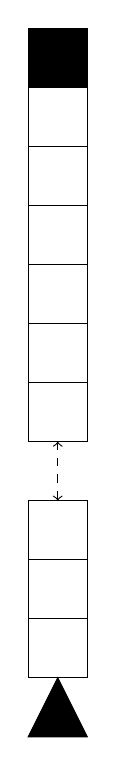
\begin{tikzpicture}
\foreach \y in {0,0.75,1.5, 3.0,3.75,4.5,5.25,6.0,6.75}{
\draw [black] (0.0, \y) rectangle ++(.75,.75);
}
\draw [dashed,<->] (0.375,2.25) -- ++(0,0.75);
\filldraw [black] (0, 7.5) rectangle ++(.75,.75); 
\filldraw [black] (0, -0.75) -- (0.375, 0) -- (0.75, -0.75) -- cycle;
\end{tikzpicture}
}
\end{columns}

\begin{equation*}
P(t, h(t))= 
 \left\{
\begin{array}{cclrcll}
P_o & [ \text{psia} ] & , & 0\; [\text{s}] < & t & \leq t^{*}(h) & [\text{s}] \\
P_o + g \frac{ h(t) - h }{ v_{l} } & [ \text{psia} ] & , &  & t & > t^{*}(h) & [\text{s}]
\end{array}\right.
\end{equation*}

\end{frame}
%---------
%---------
\begin{frame}
\frametitle{Analytic Solution}

\begin{figure}[h!t]
\centering
\includegraphics[width=0.94\textwidth]{../plots/vmpAnalytic_pdf}
\end{figure}

\end{frame}
%---------
%---------
\begin{frame}
\frametitle{Linear Solution with $\dtmax{} = \expneg{1.0}{1}$ [s]}

\begin{figure}[h!t]
\centering
\includegraphics[width=0.94\textwidth]{../plots/vmpLinear1em1_pdf}
\end{figure}

\end{frame}
%---------
%---------
\begin{frame}
\frametitle{Linear $\dt{}$ with $\dtmax{} = \expneg{1.0}{1}$ [s]}

\begin{figure}[h!t]
\centering
\includegraphics[width=0.94\textwidth]{../plots/vmpDeltaTLin1em1_pdf}
\end{figure}

\end{frame}
%---------
%---------
\begin{frame}
\frametitle{Nonlinear Solution with $\dtmax{} = \expneg{1.0}{1}$ [s]}

\begin{figure}[h!t]
\centering
\includegraphics[width=0.94\textwidth]{../plots/vmpNLN1em1_pdf}
\end{figure}

\end{frame}
%---------
%---------
\begin{frame}
\frametitle{Nonlinear $\dt{}$ with $\dtmax{} = \expneg{1.0}{1}$ [s]}

\begin{figure}[h!t]
\centering
\includegraphics[width=0.94\textwidth]{../plots/vmpDeltaTNln1em1_pdf}
\end{figure}

\end{frame}
%---------
%---------
\begin{frame}
\frametitle{Bottom Section in Nonlinear Domain}

\begin{figure}[h!t]
\centering
\includegraphics[width=0.94\textwidth]{../plots/vmpBotNln1em1_pdf}
\end{figure}

\end{frame}
%---------
%---------
\begin{frame}
\frametitle{Top Section in Nonlinear Domain}

\begin{figure}[h!t]
\centering
\includegraphics[width=0.94\textwidth]{../plots/vmpTopNln1em1_pdf}
\end{figure}

\end{frame}
%------------------------------------------------------------------------------
%------------------------------------------------------------------------------
\section[Practical Applications]{Practical Application}
%------------------------------------------------
%------------------------------------------------
\subsection[Post-Blowdown Refill Problem]{Post-Blowdown Refill Problem}
%---------
%---------
\begin{frame}[shrink=5]
\frametitle{Post-Blowdown Refill Problem}

\textbf{Purpose:} to demonstrate the use of the selective nonlinear refinement algorithm in physically relevant scenarios.

\begin{itemize}
\item{Simplified model of PWR reactor pressure vessel.}
\item{Simulation starts after blow-down stage of LOCA.}
\item{Conditions:
\begin{itemize}
\item{Section 1 $\rightarrow$ $\alpha_{l} = 1$}
\item{Downcomer: Mix of air and steam}
\item{Core: Steam}
\item{Containment @ A}
\item{Safety Injection @ B @ 25 $\displaystyle \left[ \frac{\lbm{}}{\text{s}} \right]$ @ 20 [s].}
\item{Steam Generation @ Points C \& D @ 25 [s].}
\end{itemize}
}
\end{itemize}


\end{frame}
%---------
%---------
\begin{frame}
\frametitle{Post-Blowdown Refill Model}

\begin{center}
\resizebox{0.75\textwidth}{0.75\textheight}{

\tikzsetnextfilename{images/refillComplexModel_pdf}
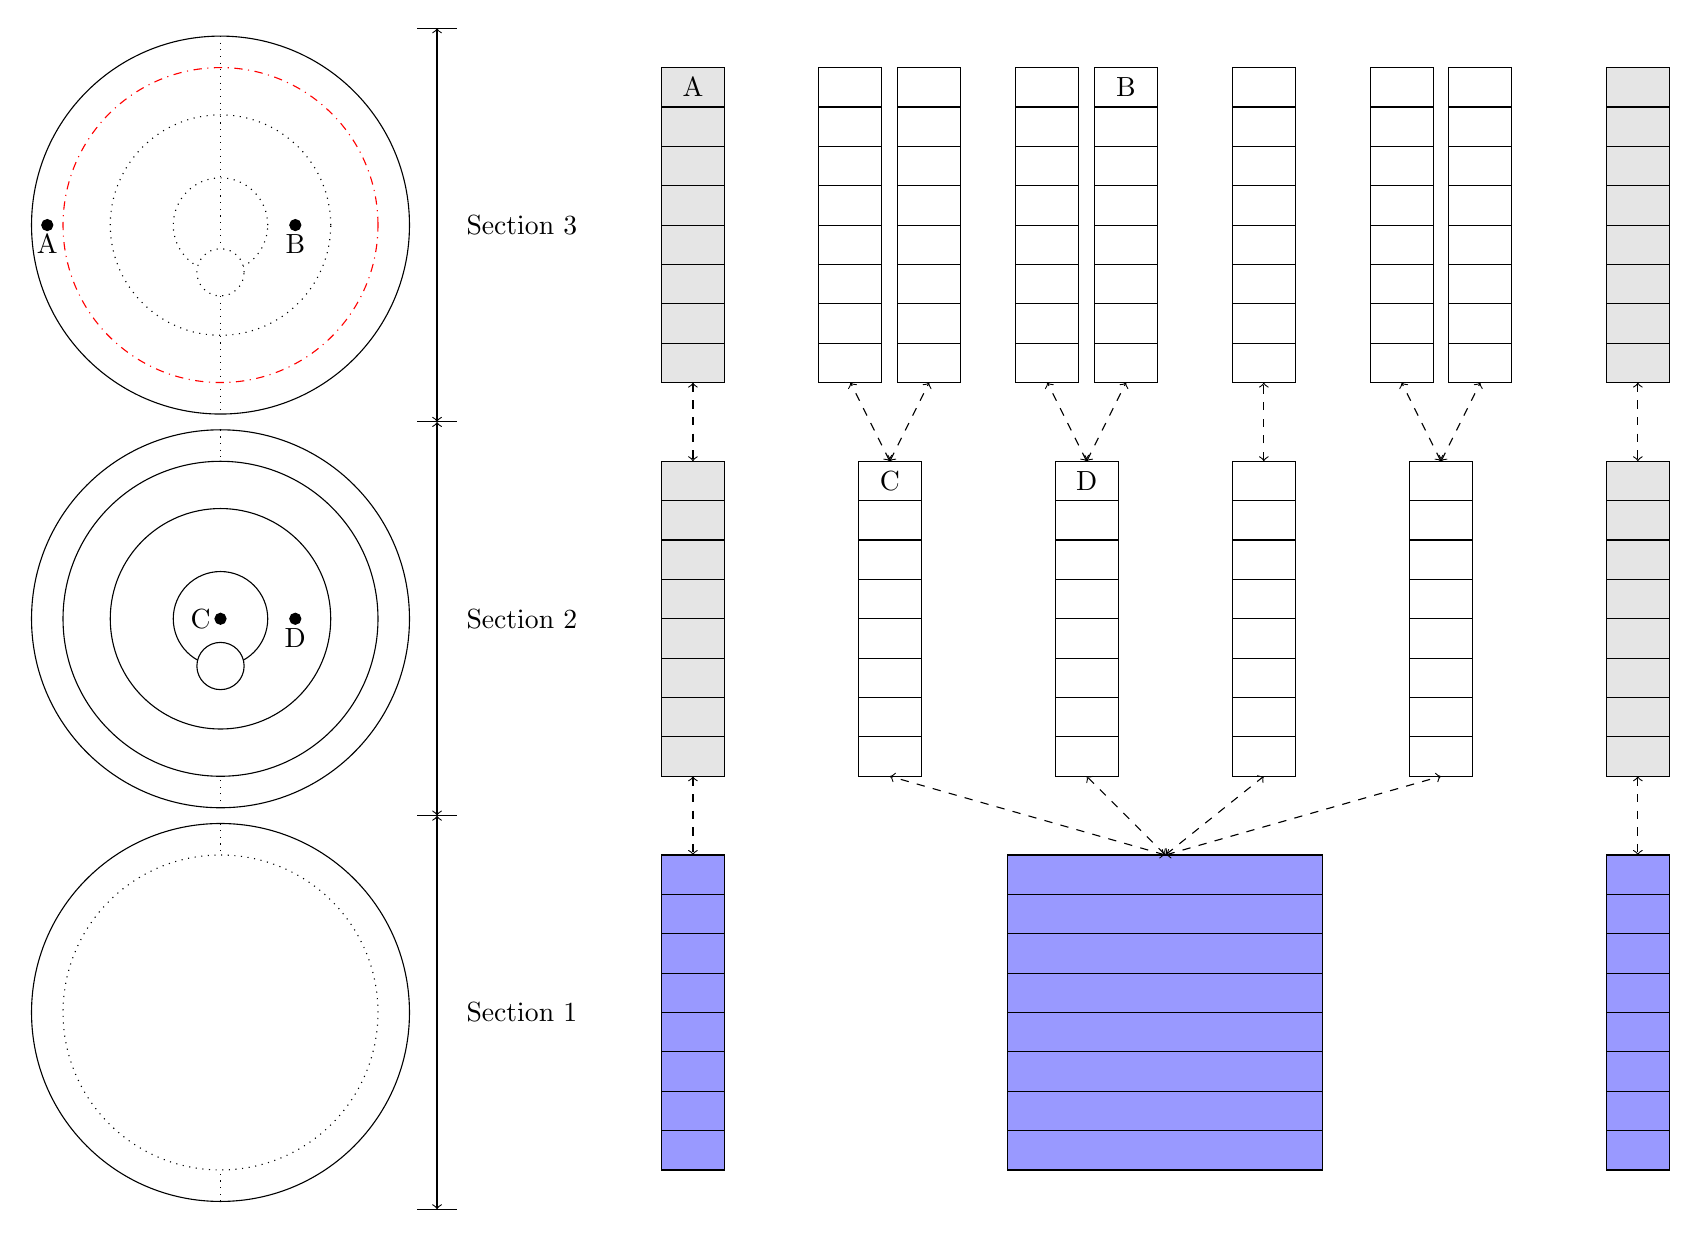
\begin{tikzpicture}

%CIRCLES
%Section 3 Flow Pattern
\draw [dotted] (0.0, 11.9) -- (0, 9.2);
\draw [dotted] (0.0, 8.6) -- (0, 7.1);
\draw [dotted] (0.0, 9.5) circle (0.6);
\draw [dotted] (0.0, 9.5) circle (1.4);
\draw [dashdotted, color=red]  (0.0, 9.5) circle (2.0);
\draw [solid]  (0.0, 9.5) circle (2.4);
\filldraw [dotted, fill=white, draw=black] (0.0, 8.9) circle (0.3);
\filldraw [black] ( 0.95, 9.5) circle (2pt) node[anchor=north]{B};
\filldraw [black] (-2.20, 9.5) circle (2pt) node[anchor=north]{A};	

%Section 2 Flow Pattern
\draw [solid] (0.0, 4.5) circle (0.6);
\draw [solid] (0.0, 4.5) circle (1.4);
\draw [solid] (0.0, 4.5) circle (2.0);
\draw [solid] (0.0, 4.5) circle (2.4);
\filldraw [fill=white, draw=black] (0.0, 3.9) circle (0.3);
\draw [dotted] (0.0, 6.9) -- (0.0, 6.5);
\draw [dotted] (0.0, 2.1) -- (0.0, 2.5);
\filldraw [black] (0.0, 4.5) circle (2pt) node[anchor=east]{C};	
\filldraw [black] ( 0.95, 4.5) circle (2pt) node[anchor=north]{D};

%Section 1 Flow Pattern
\draw [solid]  (0.0, -0.5) circle (2.4);
\draw [dotted] (0.0, -0.5) circle (2.0);
\draw [dotted] (0.0,  1.9) -- (0.0,  1.5);
\draw [dotted] (0.0, -2.9) -- (0.0, -2.5);

%Arrows & Labels
\draw (2.5,12) -- (3,12);
\draw [<->] (2.75,12) -- (2.75,7);
\draw (2.5,7) -- (3,7);
\draw [<->] (2.75,7) -- (2.75,2);
\draw (2.5,2) -- (3,2);
\draw [<->] (2.75,2) -- (2.75,-3);
\draw (2.5,-3) -- (3,-3);
\foreach \y/\ytext in {-0.5/Section 1,4.5/Section 2,9.5/Section 3}
	\draw (3,\y) node [anchor=west] {\ytext};

%RECTANGLES
% Section 3
\foreach \x in {6,18}
{
\filldraw [gray!20](\x,9.5) +(-.4,-2) rectangle ++(.4,2);
}
\foreach \x in {6,8,9,10.5,11.5,13.25,15,16,18}
{
\draw (\x,9.5) +(-.4,-2) rectangle ++(.4,2);
}
% Section 2
\foreach \x in {6,18}
{
\filldraw [gray!20] (\x,4.5) +(-.4,-2) rectangle ++(.4,2);
}
\foreach \x in {6,8.5,11,13.25,15.5,18}
{
\draw (\x,4.5) +(-.4,-2) rectangle ++(.4,2);
}
% Section 1
\filldraw [blue!40] (10,-2.5) rectangle (14,1.5);
\draw [black] (10,-2.5) rectangle (14,1.5);
\foreach \x in {6,18}
{
\filldraw [blue!40](\x,-0.5) +(-.4,-2) rectangle ++(.4,2);
\draw [black] (\x,-0.5) +(-.4,-2) rectangle ++(.4,2);
}

%Horizontal Partitions
%Section 3
\foreach \x in {6,8,9,10.5,11.5,13.25,15,16,18}
\foreach \y in {8,8.5,...,11.5}
{
\draw (\x,\y) +(-.4,0) -- ++(.4,0);
}
%Section 2
\foreach \x in {6,8.5,11,13.25,15.5,18}
\foreach \y in {3,3.5,...,6.5}
{
\draw (\x,\y) +(-.4,0) -- ++(.4,0);
}
%Section 1
\foreach \x in {6,18}
\foreach \y in {-2,-1.5,...,1.5}
{
\draw (\x,\y) +(-.4,0) -- ++(.4,0);
}
\foreach \y in {-2,-1.5,...,1.5}
{
\draw (10,\y)--(14,\y);
}

%Flow Lines
\foreach \x in {6,18}
\foreach \y in {2,7}
{
\draw [dashed,<->](\x,\y) +(0,0.5) -- ++(0,-0.5);
}
\foreach \x in {8.5,11,13.25,15.5}
{
\draw [dashed,<->](12,1.5) -- (\x,2.5);
}
\foreach \x in {8,9}
{
\draw [dashed,<->](8.5,6.5) -- (\x,7.5);
}
\foreach \x in {10.5,11.5}
{
\draw [dashed,<->](11,6.5) -- (\x,7.5);
}
\draw [dashed,<->](13.25,6.5) -- (13.25,7.5);
\foreach \x in {15,16}
{
\draw [dashed,<->](15.5,6.5) -- (\x,7.5);
}

%Labels
\draw (6,11.25) node {A};
\draw (11.5,11.25) node {B};
\draw (8.5,6.25) node {C};
\draw (11,6.25) node {D};

\end{tikzpicture}
}
\end{center}

\end{frame}
%---------
%---------
\begin{frame}
\frametitle{Steam Generation Rate}

\begin{figure}[h!t]
\centering
\includegraphics[width=0.94\textwidth]{../plots/refillSteamRates_pdf}
\end{figure}

\end{frame}
%---------
%---------
\begin{frame}
\frametitle{Downcomer and Core Effective Volume Fractions}

\begin{figure}[h!t]
\centering
\includegraphics[width=0.94\textwidth]{../plots/refillCoreVolFracDom_pdf}
\end{figure}

\end{frame}
%---------
%---------
\begin{frame}
\frametitle{Linear Solver's Net Condensation}

\begin{figure}[h!t]
\centering
\includegraphics[width=0.94\textwidth]{../plots/refillGammaLin_pdf}
\end{figure}

\end{frame}
%---------
%---------
\begin{frame}
\frametitle{Nonlinear Solver's Net Condensation}

\begin{figure}[h!t]
\centering
\includegraphics[width=0.94\textwidth]{../plots/refillGammaNln_pdf}
\end{figure}

\end{frame}
%---------
%---------
\begin{frame}
\frametitle{Dual-Domain Solver's Net Condensation}

\begin{figure}[h!t]
\centering
\includegraphics[width=0.94\textwidth]{../plots/refillGammaDom_pdf}
\end{figure}

\end{frame}
%---------
%---------
\begin{frame}
\frametitle{Maximum Condensation v. \dtmax{}}

\begin{figure}[h!t]
\centering
\includegraphics[width=0.94\textwidth]{../plots/refillMaxGamma_pdf}
\end{figure}

\end{frame}
%---------
%---------
\begin{frame}
\frametitle{Run Time Ratios}

\begin{figure}[h!t]
\centering
\includegraphics[width=0.94\textwidth]{../plots/refillRunTimeRatios_pdf}
\end{figure}

\end{frame}
%------------------------------------------------------------------------------
%------------------------------------------------------------------------------
\section[Conclusions]{Conclusions}
%------------------------------------------------
%------------------------------------------------
\subsection[Conclusions]{Conclusions}
%---------
%---------
\begin{frame}
\frametitle{Summary}

\begin{itemize}
\item{Methods that resolve nonlinearities during a timestep allow for a more timestep size insensitive solution at larger \dtmax{} than methods that do not.}
\item{A timestep size insensitive solution produced by a linearized approximation may be different than one produced by a nonlinearly convergent solver.}
\item{Not resolving localized nonlinearities can degrade the accuracy of the solution globally.}
\item{By using the domain decomposition algorithm to resolve localized nonlinearities, a simulation can achieve the accuracy and consistency of a fully nonlinear solver without its associated computational costs.}
\end{itemize}

\end{frame}
%------------------------------------------------
%------------------------------------------------
\subsection[Future Work]{Future Work}
%---------
%---------
\begin{frame}
\frametitle{Future Work}

\begin{itemize}
\item{Develop a way to adaptively determine when and where additional nonlinear iterates would be advantageous.}
\item{Investigate the computational costs of the general algorithm to determine when it would be more advantageous to include the entire domain in the nonlinear domain than it would be to use the domain decomposition algorithm.}
\item{Investigate the interaction between the nonlinear hydrodynamics and the explicit fluid-solid heat transfer.}
\item{Investigate impact of switching the governing equations upon nonlinear convergence.}
\end{itemize}

\end{frame}
%------------------------------------------------------------------------------
%------------------------------------------------------------------------------
\section*{}
%------------------------------------------------
%------------------------------------------------
\begin{frame}
\frametitle{Acknowledgments}

This research was performed under appointment to the Rickover Fellowship Program in Nuclear Engineering sponsored by Naval Reactors Division of the U.S. Department of Energy.

\end{frame}
%---------
%---------
\begin{frame}
\frametitle{Methods}
\begin{itemize}
\item{Fully Explicit Method
\begin{itemize}
\item{Lowest computational cost per timestep}
\item{Subject to sonic CFL limit: $ \dt{} \lesssim \frac{\dx{}}{|u|+|c|}$}
\end{itemize}
}
\item{Fully Implicit Method
\begin{itemize}
\item{Highest computational cost per timestep.}
\item{Not subject to CFL limit.}
\item{Nonlinearly convergent}
\item{CATHARE (Barre and Bernard, 1990)}
\end{itemize}
}
\item{Semi-Implicit Method (Liles and Reed, 1978)
\begin{itemize}
\item{Single Newton step}
\item{Subject to material Courant limit: $ \dt{} \lesssim \frac{\dx{}}{|u|}$}
\item{RELAP, TRACE, COBRA, MARS, SPACE} 
\end{itemize}
}
\end{itemize}
\end{frame}
%---------
%---------
\begin{frame}
\frametitle{Methods}
\begin{itemize}
\item{Stability-Enhancing Two-Step Method (SETS) (Mahaffy, 1982)
\begin{itemize}
\item{Multistage method}
\item{Nonlinearly convergent}
\item{Capable of exceeding material Courant limit}
\item{TRAC-M/Fortran 90, TRACE}
\end{itemize}
}
\item{Nearly Implicit Method (Trapp and Riemke, 1986)
\begin{itemize}
\item{Derivative of SETS method}
\item{Multistage method}
\item{Single Newton step}
\item{Capable of exceeding material Courant limit}
\item{RELAP}
\end{itemize}
}
\end{itemize}

\end{frame}
%---------
%---------
\begin{frame}
\frametitle{Fully Explicit Method}
Residual: $\vec{F}(\vec{x}^{n+1}) = \vec{y}(\vec{x}^{n+1}) - \vec{y}^{n} - \dt{} \vec{E}(\vec{x}^{n})$.
\begin{columns}
\column{0.45\textwidth}
\begin{itemize}
\item{Lowest per timestep computational cost.}
\item{Nonlinearities in the new-time conserved quantities.}
\item{Sonic Courant limit: $ \Delta t \lesssim \frac{\Delta x}{|u|+|c|}$}
\end{itemize}

\column{0.55\textwidth}
\begin{algorithmic}
\scriptsize
\Require $\vec{x}^{0}$ and $t^{0}$
\Set $n = 0$
\Loop \; Take a Time Step
    \Set $t^{n+1} : = t^{n} + \Delta t$
    \Calculate $\vec{F}(\vec{x}^n)$ and $\vec{J}(\vec{x}^n)$
    \Calculate $\vec{\delta x} = -\vec{J}^{-1}\vec{F}$
    \Calculate $\vec{x}^{n+1} = \vec{x}^{n} + \vec{\delta x}$ 
\EndLoop{\;$n = n+1$}
\end{algorithmic}

\end{columns}

\end{frame}
%---------
%---------
\begin{frame}
\frametitle{Fully Implicit Method}

Residual: $\vec{F}(\vec{x}^{n+1}) = \vec{y}(\vec{x}^{n+1}) - \vec{y}^{n} - \dt{} \vec{E}(\vec{x}^{n+1})$.

\begin{columns}
\column{0.45\textwidth}

\begin{itemize}
\item{Highest per timestep computational cost.}
\item{Nonlinearities in $\vec{E}(\vec{x}^{*})$.}
\item{No Courant limit.}
\item{CATHARE}
\end{itemize}

\column{0.55\textwidth}

\begin{algorithmic}
\scriptsize
\Require $\vec{x}^{0}$ and $t^{0}$
\Set $n = 0$
\Loop \; Transient Loop
    \Set $t^{n+1} : = t^{n} + \Delta t$
    \Set $k = 0$
    \Set $\vec{x}^{k} = \vec{x}^{n}$
    \Loop \; Newton Loop
		\Calculate $\vec{F}(\vec{x}^{k})$ and $\vec{J}(\vec{x}^{k})$
		\Calculate $\vec{\delta x}^k = - \vec{J}^{-1}\cdot\vec{F}$
		\BlackBox Calculate $\vec{x}^{k+1}$
		\BlackBox Terminate Loop
	\EndLoop{\;$k = k + 1$} 	
\EndLoop{\;$n = n + 1$}
\end{algorithmic}

\end{columns}
\end{frame}
%---------
%---------
\begin{frame}
\frametitle{Stability-Enhancing Two-Step Method}

\begin{columns}
\column{0.45\textwidth}

\begin{itemize}
\item{Developed to overcome material Courant limit of the semi-implicit method.}
\item{Multistage approximation to $\vec{E}(\vec{x}^{*})$.}
\item{Courant limit above the material Courant limit but not unbounded.}
\item{TRACE}
\end{itemize}

\column{0.5\textwidth}
\begin{algorithmic}
\scriptsize
\Require $\vec{x}^{0}$ and $t^{0}$
\Set $n = 0$
\Loop \; Transient Loop
    \State $t^{n+1} : = t^{n} + \Delta t$
	\Calculate $\vec{F}_1$ and $\vec{J}_1$
	\Calculate $\vec{u}^{*}$ from $\vec{\delta u}^{*} = -\vec{J}^{-1}_1\vec{F}_1$
	\Loop \; Newton Loop
		\Calculate $\vec{F}_2$ and $\vec{J}_2$
		\Calculate $\vec{\delta x} = - \vec{J}_2^{-1}\vec{F}_2$
		\Calculate $\vec{x}^{n+1} = \vec{x}^{n} + \vec{\delta x}$
	\EndLoop
	\Calculate $\vec{x}^{n+1}$ from $\vec{F}_3$.
\EndLoop{\; $n = n + 1$} 
\end{algorithmic}

\end{columns}
\end{frame}
%---------
%---------
\begin{frame}
\frametitle{Nearly-Implicit Method}

\begin{columns}
\column{0.45\textwidth}

\begin{itemize}
\item{Derivative of SETS method.}
\item{Developed to overcome material Courant limit of the semi-implicit method.}
\item{Three-stage approximation to $\vec{E}(\vec{x}^{*})$.}
\item{Courant limit above the material Courant limit but not unbounded.}
\item{Two-stage variant used in RELAP5-3D}
\end{itemize}

\column{0.5\textwidth}
\begin{algorithmic}
\scriptsize
\Require $\vec{x}^{0}$ and $t^{0}$
\Set $n = 0$
\Loop \; Transient Loop
    \State $t^{n+1} : = t^{n} + \Delta t$
	\Calculate $\vec{F}_1$ and $\vec{J}_1$
	\Calculate $\vec{\delta x}^{*} = -\vec{J}^{-1}_1\vec{F}_1$
	\Calculate $\vec{c}^{*}$ and $\vec{u}^{n+1}$
	\Calculate $\vec{F}_2$
	\Calculate $\vec{c}^{**}$ from $\vec{F}_2$
	\Calculate $\vec{c}^{n+1}$ from $\vec{F}_3$.
\EndLoop{\; $n = n + 1$}
\end{algorithmic}

\end{columns}

\end{frame}
%---------
%---------
\begin{frame}
\frametitle{Phase Transition}

\begin{itemize}
\item{Does not switch to single-phase flow conservation equations.}
\item{Minimum volume fraction for each water phase is enforced: $\alpha_{k,\text{MIN}}$ = 1.0E-9.}
\item{The two liquid water fields split the minimum presence equally.}
\item{Velocity equilibrium of fields during psuedo single-phase flow is enforced through an artificial interfacial drag.}
\item{The \ncg{} field, through its partial pressure $P_n$, is allowed to go zero.}
\end{itemize}

\end{frame}
%---------
%---------
\begin{frame}
\frametitle{Timestep Failure Mitigation and Size Selection}

\begin{itemize}
\item{Change of phasic enthalpy cannot be greater than 45 [$\frac{\text{BTU}}{\lbm{}}$].}
\item{Change in pressure cannot be greater than 20 [psia].}
\item{Change in partial pressure of the \ncg{} field cannot be greater than 20 [psia].}
\item{Thermodynamic variables would fall outside of the range of validity of the equations of state.}
\end{itemize}

\begin{equation*}
\label{eqn:time_step}
\Delta t^{n} = \max\left[ \Delta t_{\text{MIN}}, \min\left[1.2 \Delta t^{n-1}, 0.85 \Delta t_{\text{CRNT}}, \Delta t_{\text{MAX}} \right]\right]
\end{equation*}

\end{frame}
%---------
%---------
\begin{frame}
\frametitle{RELAP5-3D Semi-Implicit Coupling}

\begin{IEEEeqnarray}{rcl}
\label{eqn:si_relap}
\delta P^{n+1}_{k} = a_k & + & 
\sum_{j = 1}^{N_c} \left[ b_{k,j}n_{g,j}^{n+1} + c_{k,j}u_{g,j}^{n+1} + d_{k,j}u_{f,j}^{n+1} + e_{k,j}m_{g,j}^{n+1} \right. \nonumber \\
& + & \left. f_{k,j}m_{f,j}^{n+1} + g_{k,j}w_{g,j}^{n+1} +h_{k,j}w_{f,j}^{n+1} \right] \nonumber
\end{IEEEeqnarray}

\begin{IEEEeqnarray}{rcl}
\label{eqn:pressure_coupled}
\delta P^{n+1}_{\text{cbv}} = a_{\text{cbv}} & + & 
\sum_{j = 1}^{N_c} A_j \left[ b_{\text{cbv},j}<\alpha^n_g \rho^n_n>^{n}_{d} v_{g,j}^{n+1} \right. \nonumber \\
& + & c_{\text{cbv},j}<\alpha_g^n \rho_g^n u^n_g>_d^n v_{g,j}^{n+1} +
d_{\text{cbv},j} <\alpha_f^n \rho_f^n u_f^n>_d^n v_{f,j}^{n+1}  \nonumber \\
& + & e_{\text{cbv},j} <\alpha_g^n \rho_g^n>_d^n v_{g,j}^{n+1} +
f_{\text{cbv},j} \don{\alpha_f^n \rho_f^n}_d^n v_{f,j}^{n+1} \nonumber \\
& + & \left. g_{\text{cbv},j} <\alpha^n_g>_d^n v_{g,j}^{n+1} +
h_{\text{cbv},j} <\alpha_f^n>_d^n v_{f,j}^{n+1} \right] \nonumber
\end{IEEEeqnarray}

\end{frame}
%---------
%---------
%\begin{frame}
%\frametitle{Convergence Metrics for Flashing Problem}
%
%\begin{table}[h!t]
%\centering
%\resizebox{0.9\textwidth}{!}{
%\begin{tabular}{@{}l r@{.}l r@{.}l r@{.}l r@{.}l @{}}
%\toprule
%& \multicolumn{4}{c}{$\tilde{R}$} & \multicolumn{4}{c}{$\tilde{R}_{\text{M}}$}  \\
%$\dtmax{}$ & \multicolumn{2}{c}{Legacy} & \multicolumn{2}{c}{Nonlinear} & \multicolumn{2}{c}{Legacy}& \multicolumn{2}{c}{Nonlinear}  \\
%\midrule
%1.0    & \multicolumn{2}{c}{-} & 1&177E-3 & \multicolumn{2}{c}{-} & 6&885E-4 \\
%1.0E-1 & 5&487E-2 & 1&141E-3 & 5&044E-2 & 6&730E-4 \\
%1.0E-2 & 4&960E-2 & 3&413E-4 & 4&570E-2 & 2&511E-4 \\
%1.0E-3 & 3&172E-2 & 2&669E-4 & 2&372E-2 & 1&975E-4 \\
%1.0E-4 & 2&504E-2 & 1&346E-4 & 1&838E-2 & 8&974E-5 \\
%1.0E-5 & 2&166E-2 & 5&075E-5 & 1&922E-2 & 4&581E-5 \\
%\bottomrule  
%\end{tabular}
%}
%\end{table}
%
%\end{frame}
%---------
%---------
%\begin{frame}
%\frametitle{Convergence Metrics for Single-Phase Problem}
%
%\begin{table}[h!t]
%\centering
%\resizebox{0.9\textwidth}{!}{
%\begin{tabular}{@{}l r@{.}l r@{.}l r@{.}l r@{.}l @{}}
%\toprule
%& \multicolumn{4}{c}{$\tilde{R}$} & \multicolumn{4}{c}{$\tilde{R}_{\text{M}}$}  \\
%$\dtmax{}$ & \multicolumn{2}{c}{Legacy} & \multicolumn{2}{c}{Nonlinear} & \multicolumn{2}{c}{Legacy}& \multicolumn{2}{c}{Nonlinear}  \\
%\midrule
%1.0    & 3&149E-3 & 1&700E-3 & 1&485E-3 & 1&070E-4 \\
%1.0E-1 & 2&866E-3 & 1&700E-3 & 1&287E-3 & 1&070E-4 \\
%1.0E-2 & 3&412E-4 & 1&357E-3 & 1&417E-4 & 7&701E-5 \\
%1.0E-3 & 2&207E-4 & 4&584E-4 & 8&805E-5 & 1&178E-4 \\
%1.0E-4 & 1&672E-4 & 1&588E-3 & 1&834E-5 & 4&958E-5 \\
%1.0E-5 & 5&493E-4 & 2&758E-4 & 1&916E-5 & 8&939E-5 \\
%\bottomrule  
%\end{tabular}
%}
%\end{table}
%
%\end{frame}
%---------
%---------
\begin{frame}
\frametitle{Temporal Convergence vs Timestep Size Insensitivity}

\begin{itemize}
\item{Timestep size insensitivity: solution is insensitive to reduction of \dtmax{}.}
\item{Temporal convergence: error due to numerical approximation of temporal integral below engineering scales of interest.}
\end{itemize}

Metrics for nonlinear convergence testing:
\begin{equation*}
\tilde{R} = \frac{\int_{t^{0}}^{t^{N}} ||\tilde{\vec{F}}(\tau)||_2 \,\mathrm{d} \tau}{t^{N} - t^{0}}
\end{equation*}
\begin{equation*}
\tilde{R}_{\text{M}} = \frac{\int_{t^{0}}^{t^{N}} \,\tau\,||\tilde{\vec{F}}(\tau)||_2 \,\mathrm{d} \tau}{\int_{t^{0}}^{t^{N}} \,\tau \,\mathrm{d} \tau}
\end{equation*}

\end{frame}
%---------
%---------
\begin{frame}
\frametitle{Methods for Nuclear Thermal Hydraulic Safety Analysis}

\begin{itemize}
\item{Fully Explicit Method [COBRA-I]}
\item{Fully Implicit Method [CATHARE] (Barre and Bernard, 1990)}
\item{Semi-Implicit Method [COBRA-TF] (Liles and Reed, 1978) }
\item{Stability-Enhancing Two-Step Method (SETS) [TRACE] (Mahaffy, 1982) }
\item{Nearly Implicit Method [RELAP] (Trapp and Riemke, 1986) }
\end{itemize}

\end{frame}
%---------
%---------
\begin{frame}[shrink=5]
\frametitle{Conservation of Momentum Equations}
\begin{IEEEeqnarray}{lCl}
F^{k}_{p, l} & = & \dot{m}_{l}^{n+1, k} - \dot{m}_{l}^{n} + \frac{\dt{}}{\dx{}}\left(\sum_{i\,\in \, N_{c} } \left( \don{\alpha_l \rho_l u_l}_{\text{d}} \ave{u}_{\text{a},l} \tilde{A}\right)_{i}^{n}
 +\ave{\alpha_l}^{n}_{\text{a}} \nabla P^{\,n+1, k} - g \ave{\alpha_l \rho_l}_{\text{a}}^{n} \right. \nonumber \\
& + & \left. K^{n}_{wl}(\dot{m}_l^{n+1, k})^2 - K^{n}_{i,gl}(u^{n+1, k}_{l} - u^{n+1,k}_{g})^2 + \left[(1 - \eta)\dot{\Gamma} u^{'} + \dot{\Upsilon} u^{'}\right]^{n} \vphantom{\sum_{N_{k}}}\right) \nonumber \\
%\label{eqn:nlnGasMomentumResidual}
F^{k}_{p, g} & = & \dot{m}_{g}^{n+1,k} - \dot{m}_{g}^{n} + \frac{\dt{}}{\dx{}}\left(\sum_{i\, \in \, N_{c} } \left( \don{\alpha_g \rho_g u_g}_{\text{d}} \ave{u}_{\text{a},g}  \tilde{A}\right)_{i}^{n}  +\ave{\alpha_g}^{n}_{\text{a}} \nabla P^{\,n+1, k} - g \ave{\alpha_g \rho_g}_{\text{a}}^{n} \right.\nonumber \\
& + & \left. K^{n}_{wg}(\dot{m}_g^{n+1, k})^2 + K^{n}_{i,gl}(u^{n+1, k}_{l} - u^{n+1, k}_{g})^2 + K^{n}_{i,ge}(u^{n+1,k}_{e} - u^{n+1,k}_{g})^2 - (\dot{\Gamma} u^{'})^{n} \vphantom{\sum_{N_{k}}}\right) \nonumber\\
%\label{eqn:nlnEntMomentumResidual}
F^{k}_{p, e} & = & \dot{m}_{e}^{n+1, k} - \dot{m}_{e}^{n} + \frac{\dt{}}{\dx{}}\left(\sum_{i\, \in \, N_{c} } \left( \don{\alpha_e \rho_l u_e}_{\text{d}} \ave{u}_{\text{a},e}  \tilde{A}\right)_{i}^{n} + \ave{\alpha_{e}}^{n}_{\text{a}} \nabla P^{\,n+1, k} - g \ave{\alpha_e \rho_l}^{n}_{\text{a}} \right. \nonumber \\
& + & \left. K^{n}_{we}(\dot{m}_e^{n+1, k})^2 - K^{n}_{i,ge}(u^{n+1, k}_{e} - u^{n+1, k}_{g})^2 + \left[\eta \dot{\Gamma} u^{'} - \dot{\Upsilon} u^{'}\right]^n\vphantom{\sum_{N_{k}}}\right) \nonumber
\end{IEEEeqnarray}

\end{frame}
%---------
%---------
\begin{frame}[shrink=20]
\frametitle{Conservation of Mass and Energy Equations}

\begin{IEEEeqnarray}{lCl}
%\label{eqn:nlnNcgMassResidual}
F^{k}_{m, n} & = & V_c\left[ (\alpha_g \rho_{n})^{n+1, k} -(\alpha_g \rho_{n})^{n}\right] +\dt{} \sum_{i\, \in \,\ N_{f}}\left( \don{\alpha^{n}_g \rho^{n}_{n}}^{n+1,k}_{d} u^{n+1, k}_{g}  A_{m} \right)_{i} \nonumber \\
%\label{eqn:nlnLiqMassResidual}
F^{k}_{m, l} & = & V_c \left(\alpha_l \rho_l \right)^{n+1,k} - V_c \left(\alpha_l \rho_l \right)^{n} + \dt{} \sum_{i\,\in\,N_{f}} \left(\don{\alpha^n_l \rho^n_l}^{n+1,k}_{d} u^{n+1, k}_l A_{m} \right)_{i} + \left[(1-\eta)\Gamma + \Upsilon\right]^{n+1, k}  \nonumber  \\
%\label{eqn:nlnGasEnergyResidual}
F^{k}_{h, g} & = & V_c \left[\left( \alpha_g \rho_g h_g \right)^{n+1, k} - \left( \alpha_g \rho_g h_g \right)^{n} - \alpha^{n}_{g} ( P^{\,n+1, k} - P^{\,n} ) \right] - q^{n}_{wg} \nonumber \\
& - & \left[q_{i,v} + \Gamma h^{'}_v + q_{gl}\right]^{n+1, k} + \dt{} \sum_{i\,\in\,N_{f}} \left(\don{\alpha^{n}_g \rho^{n}_g h_g^{n}}^{n+1,k}_{d} u^{n+1, k}_g  A_{m} \right)_{i}  \nonumber  \\
%\label{eqn:nlnLiqEnergyResidual}
F^{k}_{h, l} & = & V_c\left[\left( \alpha_l \rho_l h_l \right)^{n+1,k} - \left( \alpha_l \rho_l h_l \right)^{n} - \alpha^{n}_l (P^{\,n+1,k} - P^{\,n})\right] - \left[q_{i,l} - \Gamma h^{'}_l - q_{gl}\right]^{n+1,k}    \nonumber \\
& +& \dt{} \sum_{i \, \in \, N_{f} } \left( \don{\alpha^{n}_l \rho^{n}_l h^{n}_l}^{n+1,k}_{d} u^{n+1,k}_l A_{m} + \don{\alpha^{n}_e \rho^{n}_l h^{n}_l}^{n+1,k}_{d} u^{n+1,k}_e  A_{m} \right)_{i} - q^{n}_{wl}  \nonumber  \\
%\label{eqn:nlnEntMassResidual}
F^{k}_{m, e} & = & V_c \left(\alpha_e \rho_l \right)^{n+1,k} - V_c \left(\alpha_e \rho_l \right)^{n} + \dt{} \sum_{i \, \in \, N_{f} } \left( \don{\alpha^{n}_e \rho^{n}_l}^{n+1, k}_{d} u^{n+1,k}_e  A_{m} \right)_{i} - \left[\Upsilon - \eta \Gamma \right]^{n+1, k}  \nonumber \\
%\label{eqn:nlnVapMassResidual}
F^{k}_{m, v} & = & V_c \left[\left(\alpha_g \rho_v \right)^{n+1, k} - \left(\alpha_g \rho_v \right)^{n}\right] + \dt{} \sum_{i \, \in \, N_{f} } \left( \don{\alpha^{n}_g \rho^{n}_v}^{n+1,k}_{d} u^{n+1, k}_{g} A_{m} \right)_{i} - \Gamma^{n+1, k}  \nonumber 
\end{IEEEeqnarray}

\end{frame}
%---------
%---------
\end{document}